\documentclass[%
<<<<<<< Updated upstream
11pt,%
twoside,%
titlepage,%
german,%
=======
%draft,
11pt,%
twoside,%
titlepage,%
swissgerman,%
>>>>>>> Stashed changes
headsepline%
]{scrartcl}

\usepackage{lastpage}
\usepackage{amsthm}
\usepackage{amssymb}
\usepackage{geometry}
\usepackage{graphicx}
<<<<<<< Updated upstream
\usepackage[utf8]{inputenc}
\usepackage[ngerman]{babel}
=======
\usepackage[dvipsnames]{xcolor}
\usepackage[utf8]{inputenc}
\usepackage[swissgerman]{babel}
>>>>>>> Stashed changes
\usepackage{lscape}
\usepackage[framemethod=TikZ]{mdframed}
\usepackage[most]{tcolorbox}
\usepackage{enumerate}
\usepackage{units}
\usepackage{nicefrac}
\usepackage{pgf,tikz}
<<<<<<< Updated upstream
\usetikzlibrary{arrows}
\usetikzlibrary{patterns}
\usetikzlibrary{positioning}
\usetikzlibrary{shadows}
=======
\usepackage{tikz-3dplot}
\usepackage{tkz-euclide}
\usetikzlibrary{arrows}
\usetikzlibrary{arrows.meta}
\usetikzlibrary{patterns}
\usetikzlibrary{positioning}
\usetikzlibrary{shadows}
\usetikzlibrary{quotes, angles}
>>>>>>> Stashed changes
\usepackage{colortbl}
\usepackage{hhline}
\usepackage{multirow}
\usepackage[extendedchars]{grffile}
\usepackage{caption}
\usepackage{multicol,calc}
\usepackage{blindtext}
\usepackage{pdfpages}
\usepackage{hyperref}
\usepackage{framed}

\usepackage{marginnote}
\usepackage{qrcode}
\qrset{height=9ex}

\usepackage{longtable}
\usepackage{listings}
\usepackage{wrapfig}

\usepackage{fontawesome} % Oder FontAwesome, falls du ein Augensymbol aus einer
\newcommand{\faEyeLightGray}{\textcolor{lightgray}{\faEye}} % Custom command for the gray eye icon
<<<<<<< Updated upstream
=======
\newcommand{\faReturnGray}{\textcolor{gray}{\faMailReply}} % Custom command for the gray eye icon
\usepackage{pifont} % weitere Zeichen
>>>>>>> Stashed changes

% package für plots mit dem Befehl axes
\usepackage{pgfplots}



% Command, um Tabellen-Spalten anzupassen
\newcommand{\spaltenheight}{\rule{0mm}{3ex}}
\newcommand{\spaltenwidth}{\rule{3cm}{0mm}}
\newcommand{\spaltensep}{\\[1ex]}
%\arrayrulecolor{darkgreen}
\doublerulesepcolor{white}

% colors
\definecolor{lightyellow}{rgb}{1,1,0.8}
\definecolor{Gray}{gray}{0.9}
\definecolor{lightgray}{rgb}{0.7, 0.7, 0.7}
\definecolor{darkblue}{rgb}{0,0,0.55}
\definecolor{firebrick}{rgb}{0.7,0.13,0.13}
\definecolor{seagreen}{rgb}{0.18,0.55,0.34}
\definecolor{emerald}{HTML}{50C878} % color of Definition
\definecolor{whitesmoke}{HTML}{F5F5F5} % background for environments
\definecolor{myblizzardblue}{HTML}{87CEEB} % color of Satz

% Für Definitionen im Fliesstext
\newcommand{\definition}[1]{\colorbox{emerald}{#1}}
<<<<<<< Updated upstream
=======
% Für Regeln im Fliesstext
\newcommand{\regel}[1]{\colorbox{myblizzardblue}{#1}}
% Für Merke/Achtungs im Fliesstext
\newcommand{\merke}[1]{\colorbox{firebrick}{#1}}
>>>>>>> Stashed changes
% Geogebra-Link
\newcommand{\geogebralink}{\href{https://www.geogebra.org/calculator}{\texttt{geogebra.org}}}

% Umgebungen
\theoremstyle{definition}
    \newtheorem{bsp}{Beispiel}[subsection] % Beispiele
    \newtheorem{bem}{Bemerkung}[subsection] % Bemerkungen
\theoremstyle{plain}
    \newtheorem{thm}{Theorem} % Theorem [subsection]
    \newtheorem{satz}{Satz} % Satz [subsection]

% Umgebung lsg mit dynamischer Referenzierung und Label
\newcommand{\concatueb}[1]{ueb:#1}% Definition für concatueb
\newcommand{\concatlsg}[1]{lsg:#1}% Definition für concatlsg

\newcounter{uebcounter}[section]
\renewcommand{\theuebcounter}{\thesection.\arabic{uebcounter}}  % Zählerformat: Abschnitt.Übung

\newenvironment{lsg}[1]{%
<<<<<<< Updated upstream
    \par\noindent\textbf{Notizen zu Übung \ref{\concatueb{#1}}.}%
    \label{\concatlsg{#1}}
=======
    \par\noindent\textbf{Notizen zu Übung \theuebcounter\label{\concatlsg{#1}}}
    \hfill\hyperref[\concatueb{#1}]{\faReturnGray}\par % Hyperref-Button zurück zur Übung
>>>>>>> Stashed changes
}{%
    \par%
}

\newenvironment{uebenv}[1]{%
    \refstepcounter{uebcounter}
    \par\noindent\textbf{Übung \theuebcounter.}%
    \label{\concatueb{#1}}\hfill\hyperref[\concatlsg{#1}]{\faEyeLightGray}\par
}{%
    \par
}

% Umgebung für Definitionen
\newcounter{deff}[section]\setcounter{deff}{0}
\renewcommand{\thedeff}{\arabic{section}.\arabic{deff}}

\newenvironment{cdef}[1][]{%
    \refstepcounter{deff} 
    \ifstrempty{#1}%
    % if condition (without title)
    {\mdfsetup{%
        frametitle={%
            \tikz[baseline=(current bounding box.east),outer sep=0pt]
            \node[anchor=east,rectangle,fill=emerald]
            {\strut Definition~\thedeff};}
        }%
    % else condition (with title)
    }{\mdfsetup{%
        frametitle={%
            \tikz[baseline=(current bounding box.east),outer sep=0pt]
            \node[anchor=east,rectangle,fill=emerald]
            {\strut Definition~\thedeff:~#1};}%
        }%
    }%
% for both conditions
    \mdfsetup{%
        innertopmargin=10pt,linecolor=emerald,%
        backgroundcolor=whitesmoke,%
        linewidth=2pt,topline=true,%
        frametitleaboveskip=\dimexpr-\ht\strutbox\relax%
    } 
\begin{mdframed}[]\relax}{%
\end{mdframed}}

% Farbig umrahmte Umgebung Satz
\newcounter{satzz}[section]\setcounter{satzz}{0}
\renewcommand{\thesatz}{\arabic{section}.\arabic{satzz}}

\newenvironment{csatz}[1][]{%
    \refstepcounter{satzz}
 
    \ifstrempty{#1}%
    % if condition (without title)
    {\mdfsetup{%
        frametitle={%
            \tikz[baseline=(current bounding box.east),outer sep=0pt]
            \node[anchor=east,rectangle,fill=myblizzardblue]
            {\strut Satz~\thesatz};}
        }%
    % else condition (with title)
    }{\mdfsetup{%
        frametitle={%
            \tikz[baseline=(current bounding box.east),outer sep=0pt]
            \node[anchor=east,rectangle,fill=myblizzardblue]
            {\strut Satz~\thesatz:~#1};}%
        }%
    }%
% for both conditions
    \mdfsetup{%
        innertopmargin=10pt,linecolor=myblizzardblue,%
        backgroundcolor=whitesmoke,%
        linewidth=2pt,topline=true,%
        frametitleaboveskip=\dimexpr-\ht\strutbox\relax%
    }
\begin{mdframed}[]\relax}{%
\end{mdframed}}

% kein Einzug bei neuem Abschnitt
\setlength{\parindent}{0pt} \setlength{\parskip}{1em}
\pagestyle{headings} % gemachte Einstellungen anwenden

% Titelblatt setzen
\subject{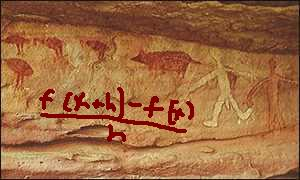
\includegraphics[width=0.618\textwidth]{pictures/cave.jpg}}
\title{Differentialrechnung}
\subtitle{The Core of the Whole Business}
\author{}
\date{}
\lowertitleback{
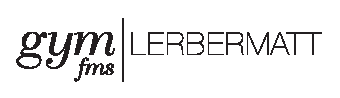
\includegraphics[height=1cm]{pictures/gymfmslerbermattlogo.eps}
\hfill%\copyright%
{\begin{tikzpicture}
  % Draw the rounded rectangle and clip the image to it
  \clip [rounded corners=5mm] (0,0) rectangle (1,1); % Adjust dimensions as needed
  \node at (0.5,0.5) {\includegraphics[width=1cm]{pictures/teacher_me_caricatur.png}}; % Adjust width and center image
\end{tikzpicture}}
}

\begin{document}
\maketitle
\tableofcontents
\cleardoublepage

\section{Tangenten- und Flächenproblem}
Die Mathematik der Antike hat ihrer Nachwelt zwei klassische Probleme überliefert: das \emph{Tangentenproblem} und das \emph{Flächenproblem}.

\begin{itemize}
\item Die Konstruktion einer Tangente an einen Kreis ist relativ einfach. Sie versagt aber schon, wenn man versucht, eine Tangente an eine Ellipse zu konstruieren. Die griechischen Geometer hatten für die Ellipse ein neues Verfahren erdacht, das aber schon wieder bei einer anderen Kurve, der Parabel, versagte. Die Konstruktion der Parabeltangente liess sich nicht auf die Hyperbel übertragen; man musste also für jede Kurve eine ganz neue Konstruktion ersinnen. Wenn nur wenige Kurven bekannt sind, besteht kein Anlass, nach einer allgemeinen Methode zu suchen. Die Situation änderte sich aber schlagartig, als zu Beginn des 17. Jahrhunderts die analytische Koordinatengeometrie entstand und somit beliebig viele Kurven zu untersuchen waren. Jetzt wurde eine universelle Methode verlangt, die es ermöglicht, den Verlauf der Tangente für jede beliebige Kurve zu studieren.
\end{itemize}

\begin{itemize}
\item Das Flächenproblem bestand darin, den Inhalt einer durch Kurven begrenzten Fläche zu berechnen. Zu diesem Problem leistete vor allem \textsc{Archimedes} (287 -- 212 v.u.Z) Hervorragendes. Seine Methode, die Exhaustionsmethode, bestand darin, die zu berechnende Fläche durch eine Folge von Flächen mit schon bekanntem Inhalt auszuschöpfen. Wenn man das Flächenproblem gelöst hat, fällt die Berechnung des Volumens eines Körpers nicht mehr so schwer. Viele spezielle Flächen und Körper konnten so durch teilweise raffinierte Zerlegungen berechnet werden. Aber auch hier existierte noch keine universelle Methode.
\end{itemize}

\clearpage

\section{Historisches zur durchschnittlichen Änderungsrate}

Nichts entgeht der Veränderung. Alles wächst oder schrumpft, erwärmt sich oder kühlt sich ab, wechselt die Stellung, die Farbe oder die Zusammensetzung. Die Fauna und die Flora liefern beliebig viele Beispiele. Selbst Felsen dehnen sich in der Sonne aus und ziehen sich im Schatten zusammen.

Der Mathematik der Antike gelang es nicht, veränderliche Grössen mathematisch zu erfassen. Ihre Mathematik war, bis auf wenige Ausnahmen, eine feste und stillstehende Welt. Andererseits zeigt dies, dass es sehr schwer ist, einen Veränderungsprozess zu analysieren und das dahinterstehende Naturgesetz zu finden.

Erst im 16. und 17. Jahrhundert war die Zeit reif, den allgemeinen Begriff der veränderlichen Grösse in die Mathematik aufzunehmen.

Für die Anwendungen der Mathematik standen Probleme der Geodäsie, der Astronomie, des Artilleriewesens, der Schifffahrt, des Kanalbaus, der maschinellen Ausrüstung von Manufakturen im Vordergrund. Die Uhren mussten enorm verbessert werden. \textsc{Leonardo da Vinci} machte sich sogar schon Gedanken über Flugmaschinen, Unterseeboote und Wagen, die ohne Zugtiere fahren konnten.
Die Mathematik sollte vor allem mechanische Bewegungsabläufe --- Planetenbewegungen, Fallbewegungen, Bewegungen gegeneinander beweglicher Maschinenteile --- erfassen und theoretisch beschreiben können.
Der neuen Mathematik des 16. und 17. Jahrhunderts gelang es, mit denselben Methoden sowohl das Tangentenproblem als auch das Flächenproblem, als auch die Bewegungsprobleme zu lösen! Sie konnte gleichzeitig die Verwandtschaft und die Gleichartigkeit all dieser Probleme aufzeigen. Auf diesen Lösungen aufbauend konnten weitere Probleme, die die naturwissenschaftliche Entwicklung immer weiter vorantrieben, bewältigt werden.

\textsc{Ren\'e Descartes} (1596 -- 1650) gelang es, die gegenseitige Abhängigkeit von veränderlichen Grössen --- ausgedrückt durch eine Gleichung oder eine Funk\-tion --- in einem Koordinatensystem graphisch darzustellen.
Weiterhin konnten die einzelnen Zustände einer Bewegung sichtbar gemacht und genau studiert werden.
Es fehlte aber noch die klare Erfassung des Funk\-tions\-begriffes und eine auf veränderliche Grössen zugeschnittene Rechentechnik.
In der zweiten Hälfte des 17. Jahrhunderts schufen dann \textsc{Isaac Newton} (1643 -- 1727) und \textsc{Gottfried Wilhelm Leibniz} (1646 -- 1716) unabhängig voneinander etwas für die bisherige Mathematik völlig Neues, das die analytische Koordinatengeometrie von \textsc{Descartes} mit der von \textsc{Archimedes} stammenden Exhaustionsmethode verband.

\begin{figure}
\begin{center}
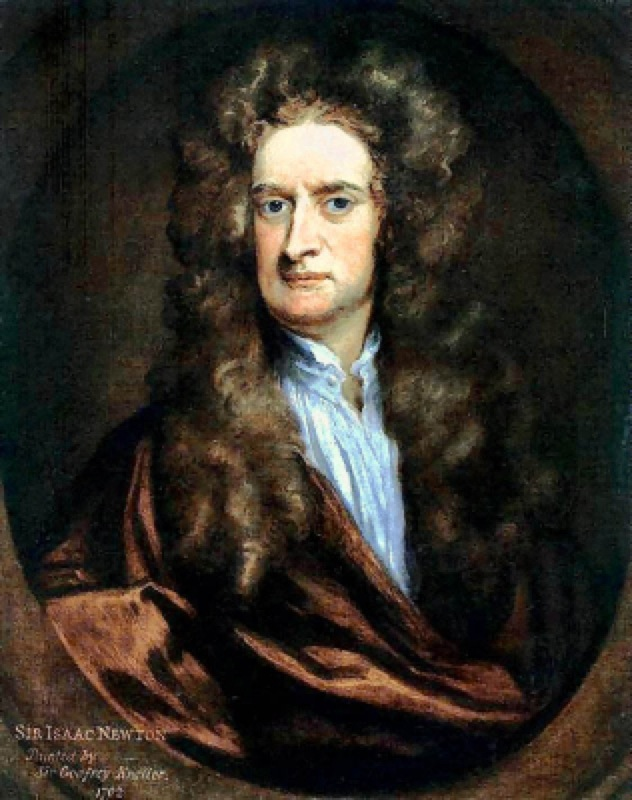
\includegraphics[width=0.4\textwidth]{pictures/newton}\hspace*{0.062\textwidth}
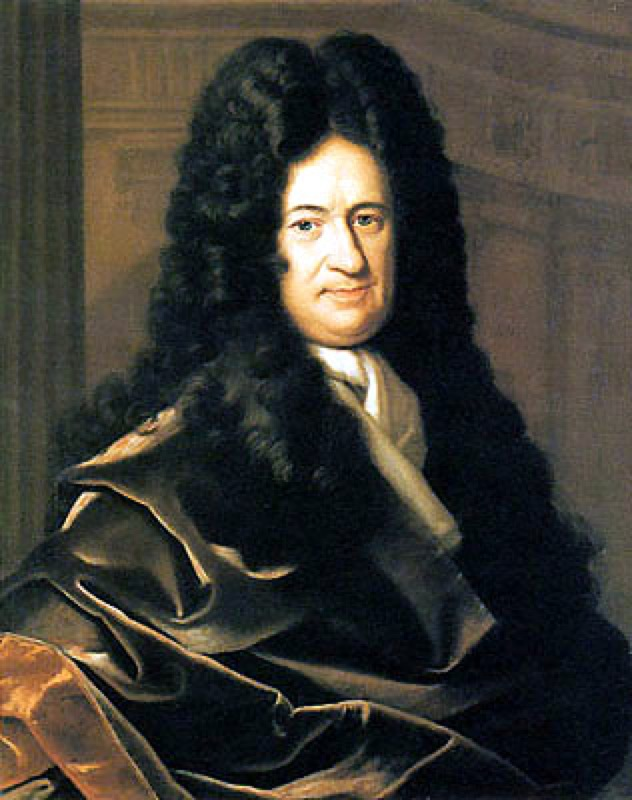
\includegraphics[width=0.4\textwidth]{pictures/leibniz}
\caption{\textsc{Sir Isaac Newton} und \textsc{Gottfried Wilhelm Leibniz}}
\end{center}
\end{figure}
Dieses neue Gebiet der Mathematik heisst heute Infinitesimalrechnung oder \emph{Analysis} oder Differenzial- und Integralrechnung oder im englischen Sprachraum \emph{Calculus}.

Die Differenzialrechnung, die das Tangentenproblem löst, bildet unter anderem die Grundlage der mechanischen Bewegungen. Mit ihr kann beispielsweise der Physiker oder Techniker aus einer gegebenen Bahnkurve für jeden Zeitpunkt die augenblickliche Geschwindigkeit ermitteln. Später eroberte sich die Differenzialrechnung immer mehr Anwendungsgebiete; zum Beispiel ist sie für die heutigen Wirtschaftswissenschaften unentbehrlich geworden.

Mit der Integralrechnung, die das Flächenproblem löst, konnte man bald nach ihrer Entdeckung auch die Bogenlänge eines Kurvenstückes oder den Rauminhalt und die Oberfläche eines krummflächig begrenzten Körpers berechnen, aber auch viele physikalische Begriffe, wie zum Beispiel Schwerpunkt, Trägheitsmoment, Arbeit etc. mathematisch erfassen. Als besonders nützlich erwies sich die Integralrechnung zu der Zeit, als die Kohle als Energiequelle die Arbeit des Menschen und des Lasttiers zu ersetzen begann. Mit ihr konnte man nämlich die Leistung und den Wirkungsgrad von Maschinen berechnen. Später wurde die Integralrechnung auch zur Grundlage der Chemie der Energiestoffe (Thermodynamik).

\clearpage

\section{Gedanken zur momentanen Änderungsrate}
Bei einer veränderlichen Situation ist nicht nur der augenblickliche Zustand von Interesse, vielmehr interessiert oft, mit welcher Geschwindigkeit sich die Situation ändert. Für die Wettervorhersage ist nicht allein die Grösse des Luftdrucks wichtig, sondern vor allem, wie stark der Druck je Stunde steigt oder fällt. Für den Wirtschaftswissenschaftler ist neben dem Marktpreis eines Produktes von besonderer Wichtigkeit, wie schnell sich der Preis mit der Zeit ändert (Teuerungsrate).
Die Infinitesimalrechnung von \textsc{Newton} und \textsc{Leibniz} kann diese und ähnliche Fragen mit zwei neuen Verfahren, der Differenziation und der Integration, beantworten.

\subsection{Von der durchschnittliche zur momentanen Änderungsrate}

Wir betrachten eine beliebige, zeitlich veränderliche Situation, deren einzelne Zustände durch die Funktion $f(t)$
beschrieben werden können. Man kann relativ einfach eine \emph{durchschnittliche} Än\-derungs\-ge\-schwin\-dig\-keit des Funktionswertes angeben, indem man die zu zwei bestimmten Zeitpunkten $t_1$ und $t_2$ gebildete Differenz der zugehörigen Funktionswerte $f(t_1)$ und $f(t_2)$ durch die Zeitspanne dividiert. Wir erinnern uns:
$$\overline{v}=\frac{\text{Änderung von }f(t)}{\text{Änderung von }t}=\frac{f(t_2)-f(t_1)}{t_2-t_1}=\frac{\Delta f}{\Delta t}$$
Mit der Differenziation kann man jedoch die \emph{momentane} Än\-derungs\-ge\-schwin\-dig\-keit des Funktionswertes zu einem beliebigen Zeitpunkt $t$ berechnen. Wie man dies mathematisch Umsetzt, darum soll es im Folgenden gehen.

Man bezeichnet üblicherweise einen Zuwachs der Variablen $t$ mit $\Delta t$ und die entsprechende Änderung des Funktionswertes zwischen den Zeitpunkten $t$ und $t+\Delta t$ mit $\Delta f$.
\begin{figure}
\centering
\scalebox{1.3}{
\begin{tikzpicture}[line cap=round,line join=round,>=triangle 45,x=0.55cm,y=0.55cm]
\draw[->,color=black] (-0.72,0) -- (12.46,0);
\foreach \x in {,1,2,3,4,5,6,7,8,9,10,11,12}
\draw[shift={(\x,0)},color=black] (0pt,-2pt);
\draw[color=black] (12.18,0.08) node [anchor=south west] {$t$};
\draw[->,color=black] (0,-1.42) -- (0,4.6);
\foreach \y in {-1,1,2,3,4}
\draw[shift={(0,\y)},color=black] (2pt,0pt) -- (-2pt,0pt);
\draw[color=black] (0.1,4.2) node [anchor=west] {$y$};
\clip(-0.72,-1.42) rectangle (12.46,4.6);
\draw[line width=1.2pt,color=seagreen, smooth,samples=100,domain=-0.72:12.46] plot(\x,{0-(0.02)*(\x-2)*(\x+2)*(\x-11)});
\draw (2.0,3.3) node[anchor=north west] {$y=f(t)$};
\draw [dotted] (2.98,0.78)-- (3,0);
\draw (2.98,0.78)-- (9,0.8);
\draw [dotted] (9,0.8)-- (9,0);
\draw (2.7,0.02) node[anchor=north west] {$t$};
\draw (8.0,0.02) node[anchor=north west] {$t+\Delta t$};
\draw (5.82,0.9) node[anchor=north west] {$\Delta t$};
\draw (9,0.78)-- (9,3.08);
\draw (8.8,1.9) node[anchor=north west] {$\Delta f$};
\fill [color=firebrick] (2.98,0.78) circle (1.5pt);
\fill [color=firebrick] (9,3.08) circle (1.5pt);
\end{tikzpicture}
}
\caption{durchschnittliche Steigung $\frac{\Delta f}{\Delta t}$}
\end{figure}
Da Zähler und Nenner jeweils Differenzen sind, heisst der Bruch \definition{Differenzenquotient}. Jetzt braucht man nur zu verfolgen, was mit dem Bruch $\frac{\Delta f}{\Delta t}$ geschieht, wenn $\Delta t$ gegen Null strebt. Zu Beginn gibt der Differenzenquotient die durchschnittliche Ände\-rungs\-ge\-schwindig\-keit des Funktionswertes zwischen den Zeitpunkten $t$ und $t+\Delta t$ an. Wenn nun $\Delta t$ gegen Null strebt, so strebt $\Delta f$ auch gegen Null. Der  Differenzenquotient $\frac{\Delta f}{\Delta t}$ kann jedoch existieren und muss nicht unbedingt gegen Null streben. Dieser Grenzwert ist, falls er existiert, die augenblickliche Änderungsgeschwindigkeit des Funktionswertes zum Zeitpunkt $t$.
Man schreibt dafür
$$\frac{\mathrm{d}f}{\mathrm{d}t}=\lim_{\Delta t\to0}\frac{\Delta f}{\Delta t}$$
und nennt diesen Grenzwert \definition{Differenzialquotient}.

Die \definition{Integration} ist in gewisser Weise die Umkehrung der Differenziation, etwa in der Art, wie die Addition und Subtraktion oder Multiplikation und Division Umkehrungen voneinander sind. Bei der Integration sucht man eine Funktion, deren Differenzialquotient $q(t)$ bekannt ist. Man nennt diese Funktion das Integral von $q(t)$ und
schreibt
$$\int q(t)\,\mathrm{d}t$$
(integrare: lat. wiederherstellen).
Kennt man zum Beispiel bei einer Autofahrt die zu\-rück\-ge\-legte Wegstrecke als Funktion der Zeit, so gibt der Differenzialquotient für einen bestimmten Zeitpunkt die momentane Geschwindigkeit an. Kennt man die Geschwindigkeit als Funktion der Zeit, so kann man mit Integration die zwischen zwei bestimmten Zeitpunkten zurückgelegte Wegstrecke berechnen.

\subsection{Das Gesetz des freien Falls nach Galilei}

Nach jahrelangen Experimenten und vielen theoretischen Anläufen konnte \textsc{Galilei} 1585 die Gesetze des freien Falls aufstellen: Ein auf die Erde herabfallender Körper legt in der Zeit t den Weg
$$s(t)=4.9 t^2$$
zurück ($t$ in Sekunden, $s(t)$ in Meter); nach der Zeit $t$ hat der Körper die Geschwindigkeit $v(t)=9.8t$ ($v(t)$ in $\unitfrac{m}{s}$); seine Beschleunigung ist zu jedem Zeitpunkt konstant, nämlich $\unitfrac[9.8]{m}{s^2}$.

Mit der von \textsc{Newton} und \textsc{Leibniz} entdeckten Infinitesimalrechnung braucht man nur die Wegstreckenfunktion
$s(t)=4.9t^2$ zu kennen. Die Geschwindigkeit ist die Änderung des Weges relativ zur Zeit, also der Differenzialquotient
$$\lim_{\Delta t\to0}\frac{\Delta s}{\Delta t}=\lim_{\Delta t\to0}\frac{4.9(t+\Delta t)^2-4.9t^2}{\Delta t}$$
und damit
$$v(t)=\lim_{\Delta t\to0}4.9\cdot 2t+4.9\Delta t=9.8t.$$

\begin{uebenv}{galilei}
    Rechne nach, dass aus $s(t)$ tatsächlich mit Hilfe des Differentialquotienten $v(t)$ folgt.
\end{uebenv}

Die Beschleunigung $a(t)$ ist die Veränderung der Geschwindigkeit relativ zur Zeit, also der Differenzialquotient
$$\lim_{\Delta t\to0}\frac{\Delta v}{\Delta t}=\lim_{\Delta t\to0}\frac{9.8(t+\Delta t)-9.8t}{\Delta t}=9.8$$
Die Beschleunigung ändert sich nicht mehr mit der Zeit, sie ist konstant. Das hinter dem freien Fall stehende Naturgesetz, dass jeder frei fallende Körper mit der konstanten Beschleunigung von $\unitfrac[9.8]{m}{s^2}$ auf die Erde fällt, tritt klar und ohne grossen Aufwand ans Licht.

\subsection{Leibniz oder Newton?}

Noch heute wird \textsc{Newton} als der grösste Physiker und als einer der grössten Mathematiker bezeichnet. \textsc{Albert Einstein} schrieb:
\begin{quote}
\glqq Für \textsc{Newton} war die Natur ein offenes Buch, dessen Buchstaben er mühelos lesen konnte.\grqq
\end{quote}
Newton selbst sagte: 
\begin{quote}
\glqq Mir selbst kommt es vor, als wäre ich wie ein Knabe gewesen, der am Strand des Meeres spielt und sich damit vergnügt, hier und da einen glatteren Kiesel oder eine schönere Muschel zu finden, während der grosse Ozean der Wahrheit unentdeckt vor mir lag.\grqq
\end{quote}
An anderer Stelle erklärt er bescheiden, er habe nur deshalb weiterschauen können, weil er auf den \glqq Schultern von Riesen\grqq\ gestanden habe. Damit meinte er in erster Linie \textsc{Archimedes} (287 -- 212 v.u.Z), \textsc{Johannes Kepler} (1571 -- 1630), \textsc{Galileo Galilei} (1564 -- 1642), \textsc{Blaise Pascal} (1623 -- 1662), \textsc{Pierre de Fermat} (1601 -- 1665) und \textsc{Ren\'e Descartes} (1596 -- 1650).

Newtons Ergebnisse (Axiome, freier Fall, Planetenbewegung, Gravitation, Berechnung der Gezeiten, \dots), die schon 1671 in einem druckfertigen Manuskript vorlagen, erschienen erst 1687 in seinem Buch \glqq Philosophiae naturalis principia mathematica\grqq, in dem die Bewegungsgesetze formuliert und damit die Grundlagen der Mechanik gelegt wurden. Erst durch Einstein wurde zu Beginn des 20. Jahrhunderts die Newton'sche Physik in einen noch tieferen Zusammenhang, den der Relativitätstheorie, eingebettet.

\textsc{Leibniz} war nicht nur ein bedeutender Mathematiker. Er sprach schon mit 12 Jahren griechisch und lateinisch, war Philosoph, Historiker, Jurist und Diplomat. Er lieferte wesentliche Beiträge zur Mechanik, Biologie und theoretischen Logik; er gründete 1700 die Berliner Akademie der Wissenschaften, war Erfinder einer Rechenmaschine, einer Universalsprache. Er machte unzählige alchemistische Versuche, kümmerte sich um Wasserförderung in den Bergwerken, Seidenraupenzucht und technische Verbesserungen von Maschinen. \textsc{Leibniz} war ein Universalgenie. 1675 gelingt \textsc{Leibniz}, unabhängig von \textsc{Newton}, die Entdeckung des \glqq Calculus\grqq, wie er seine Version der Infinitesimalrechnung nannte. Er veröffentlichte bereits ab 1684 seine Ergebnisse. Dies führte denn auch zu einem hässlichen Prioritätsstreit.
\begin{figure}
    \centering
    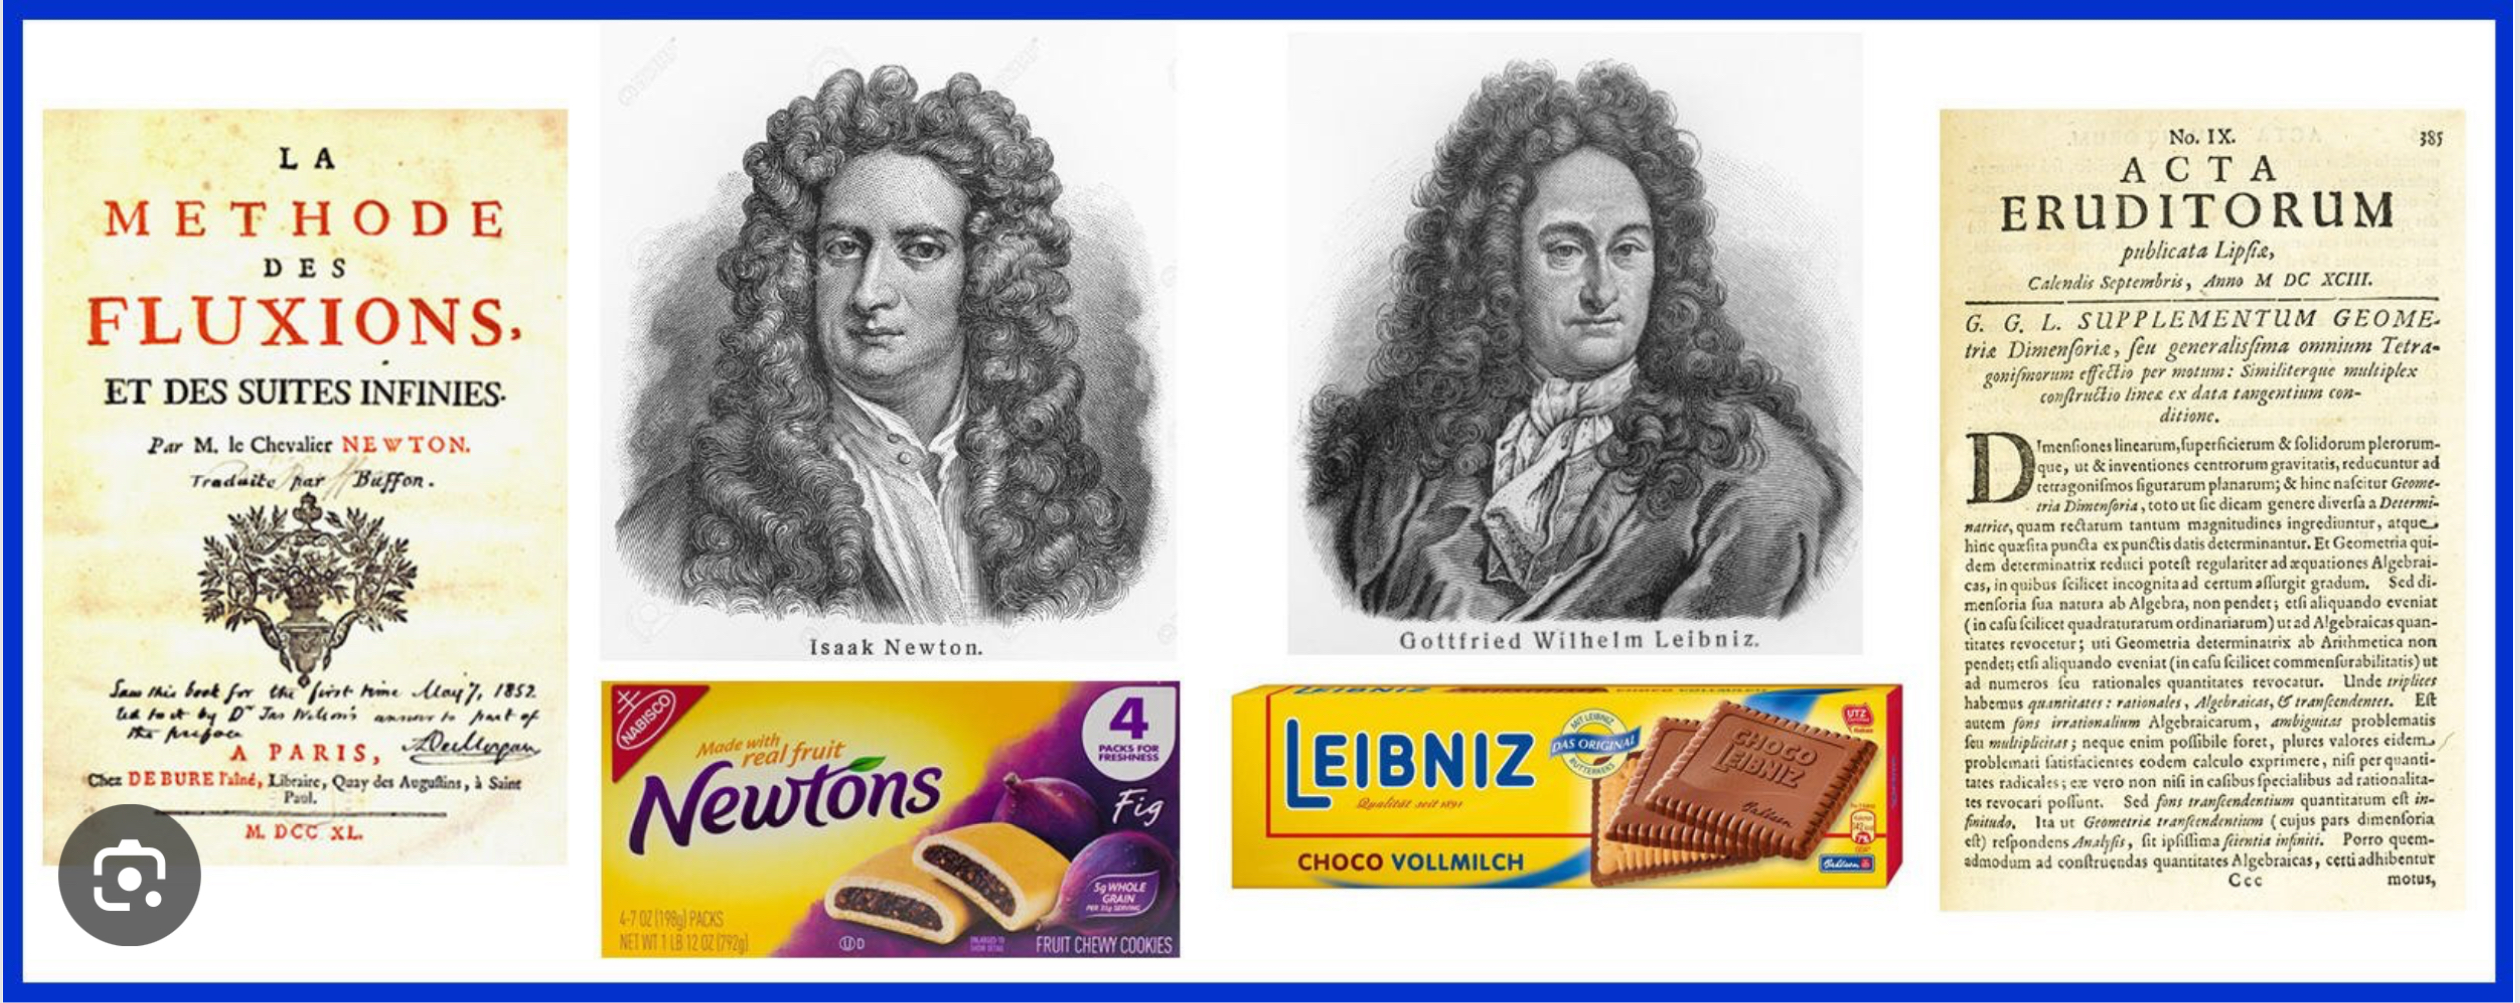
\includegraphics[width=0.62\textwidth]{pictures/newton_and_leibiz.jpeg}
    \caption{both have biscuits named after them}
    \label{fig:leibnizandnewton}
\end{figure}
Im diametralen Gegensatz zu seinem Rivalen \textsc{Newton}, der 1705 geadelt und 1727 feierlich mit einem Staatsbegräbnis in der Londoner Westminster Abtei beigesetzt wurde, war \textsc{Leibniz} bei seinem Fürsten in Ungnade gefallen und starb einsam und völlig verarmt.

\subsection{Die Leibniz-Notation}

Die rasche Verbreitung der Leibniz'schen Methoden und ihrer weitgefächerten Anwendungen auf dem Kontinent ist vor allem seiner genialen Wahl der Bezeichnungen und Symbole zu verdanken. Sein Notationssystem
$$\frac{\mathrm{d}y}{\mathrm{d}x}$$
für den Differenzialquotienten,
$$\int y\,\mathrm{d}x$$
für das Integral, wird noch heute so benutzt. Mit dieser Schreibweise war es möglich, Ergebnisse herzuleiten, ohne die tieferen Zusammenhänge zu verstehen.
So leicht macht es uns die Natur nun doch nicht, da gerade in Naturprozessen der Zufall eine grosse Rolle spielt. Dennoch gab es schon Zeitgenossen von Newton und Leibniz, die bereits an den Gesetzen der Wahrscheinlichkeitsrechnung arbeiteten, um den Zufall mathematisch erfassen zu können.

\subsection{Das Teilgebiet Analysis}

An der weiteren Entwicklung der Infinitesimalrechnung sind vor allem die Basler Mathematiker \textsc{Jakob} und \textsc{Johann Bernoulli} (1654 -- 1705, 1667 -- 1748) beteiligt. Von \textsc{Johann Bernoulli} stammt auch die Bezeichnung \glqq Integral\grqq. Beide Brüder waren Anhänger \textsc{Leibniz} und \textsc{Newton} gegenüber eher feindlich gesinnt.

Den wahren Durchbruch der Infinitesimalrechnung in den Naturwissenschaften und insbesondere der Mechanik aber erreichte der in Riehen geborene \textsc{Leonhard Euler} (1707 -- 1783). 1979 wurde ihm zu Ehren die bis 1997 gebräuchliche 10-Franken Note gestaltet.
Auf der Vorderseite erkannte man eine Zeichnung des idealen \glqq Zahn-Profils\grqq\ eines Zahnrades, eine von Eulers zahlreichen Entdeckungen. Den Hintergrund bildeten Diagramme, die \textsc{Euler} zur Darstellung logischer Schlüsse verwandte. Die drei Motive auf der Rückseite zeigten: Eine von Euler auf Grund von Berechnungen entworfene Wasserturbine, deren Grundidee noch heute bei modernen Turbinen in den Kohle- und Kernkraftwerken verwendet wird, ein Schema eines Strahlengangs durch ein System von Linsen, und eine Darstellung unseres Sonnensystems im Zusammenhang mit Eulers Mondtheorie, die für die Schifffahrt wichtigen Tafeln der Mondbewegung enorm verbesserte.

Eulers gesammelte Werke, die seit Jahrzehnten in Basel und Leningrad neu herausgegeben werden, umfassen bis jetzt etwa 100 Quartbände. Euler gilt als der letzte Mathematiker, der noch die gesamte \glqq zeitgenössische\grqq\ Mathematik beherrschte. Zum Vergleich: Heute kennt ein guter Mathematiker weniger als  0.1\% der gesamten Mathematik.

Im 19. Jahrhundert waren es neben \textsc{Lagrange} vor allem \textsc{Pierre Simon Laplace} (1749 -- 1823), \textsc{Adrien Marie Legendre} (1752 -- 1833), \textsc{Augustin Louis Cauchy} (1789 -- 1864), \textsc{Carl Friedrich Gauss} (1777 -- 1855), \textsc{Bernhard Riemann} (1826-1866) und \textsc{Karl Weierstrass} (1815 -- 1897), die eine strenge Begründung und einen weiteren Ausbau der Infinitesimalrechnung erreichten. Von diesen Analytikern stammt der Name \definition{Analysis}.

\begin{figure}
\begin{center}
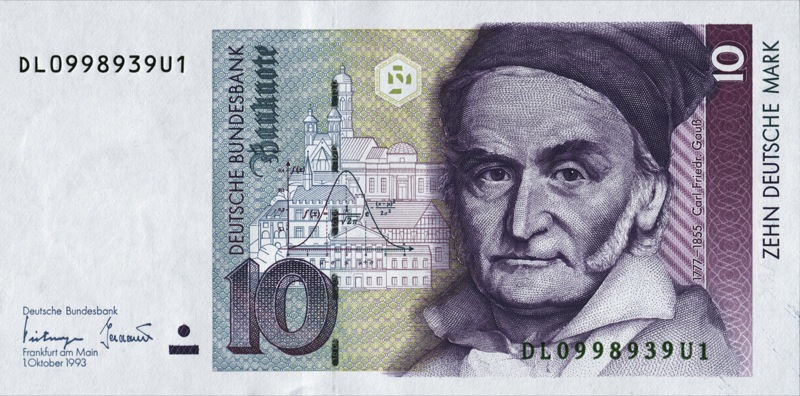
\includegraphics[width=0.618\textwidth]{pictures/gauss}
\caption{10 DM Note: \textsc{Carl Friedrich Gauss}}
\end{center}
\end{figure}

Die Arbeiten der Analytiker des 19. Jahrhunderts haben gezeigt, dass die ganze Infinitesimalrechnung auf nur fünf grundsätzlichen, klaren mathematischen Ideen beruht:

\begin{itemize}
\item Funktion
\item Behandlung des Krummen via Approximation durch Gerades
\item Konvergenz und Grenzwert
\item Differentiation
\item Integration
\end{itemize}

Dadurch ist heute die Infinitesimalrechnung für jeden interessierten Menschen zugänglich geworden. Man darf aber nicht den Schluss ziehen, dass die Entwicklung der Analysis im 19. Jahrhundert abgeschlossen worden wäre. Gegenwärtig werden in den verschiedenen Teilgebieten der Analysis jährlich mehr als 1000 Arbeiten veröffentlicht.

\subsection{Recap Differenzenquotient}
Bei vielen funktionalen Zusammenhängen ist nicht nur interessant, welche Werte eine Funktion $f$ annimmt und ob sie stetig ist, sondern auch, wie rasch bzw. stark die Funktionswerte $y=f(x)$ zu- oder abnehmen, wenn sich die $x$-Werte ändern.

\begin{cdef}[Differenzenquotient]
Der Differenzenquotient
\marginnote{
\qrcode{
https://www.youtube.com/watch?v=J0FCAuTM9pA}
}
$$\frac{f(x_0+h)-f(x_0)}{h}=\frac{\Delta y}{\Delta x}$$
gibt die durchschnittliche Änderung der Funktion $f$ im Intervall $[x_0,x_0+h]$ an.
\end{cdef}

Mit ihm erhält man eine erste grobe Aussage über das Änderungsverhalten der Funktion $f$. Dieser Differenzenquotient kann je nach Funktion verschiedene Bedeutungen haben.

\begin{bsp}\label{bspsteigungswinkel}
Bei
\marginnote{
\qrcode{
https://www.youtube.com/watch?v=BOGpb1yyD-E}
}
einer ansteigenden Strasse wird der Differenzenquotient
$$\frac{f(x_0+h)-f(x_0)}{h}=\tan(\alpha)=m.$$
Er entspricht also der durchschnittlichen Steigung des betrachteten Strassenstücks.
\end{bsp}

\begin{uebenv}{koenizberg}
Köniz liegt auf einer Höhe von 610 M.ü.M. Berechne die durchschnittliche Steigung des Könizbergs (höch\-ster Punkt 674 M.ü.M) in Prozent und berechne den Steigungswinkel, wenn die beiden Messungen horizontal $\unit[700]{m}$ auseinander liegen.
\end{uebenv}

\begin{bsp}\label{bspradioaktiv}
Beim radioaktiven Zerfall verringert sich die Anzahl der radioaktiven Kerne allmählich. Dementsprechend nimmt die Strahlung jedes radioaktiven Präparats im Laufe der Zeit ab. Die Aktivität sinkt innerhalb der sogenannten \definition{Halbwertszeit} auf die Hälfte ihres Ausgangswerts. Da radioaktive Materialen aufgrund ihrer ausgesendeten Strahlung leicht geortet werden können, dienen radioaktive Isotope in vielen Bereichen der Physik, Chemie, Biologie, Medizin und Technik als Indikatoren. Beispielsweise kann man mit Jod (J-131), das dem Organismus in geringer Menge zugeführt wird, Stoffwechselvorgänge verfolgen und allfällige Störungen feststellen. Das folgende Diagramm zeigt den Zerfall von J-131, dessen Halbwertszeit 8 Tage beträgt.

\begin{figure}
\begin{center}
\scalebox{0.9}{
\begin{tikzpicture}[line cap=round,line join=round,>=triangle 45,x=0.25cm,y=4.5cm]
\draw [color=lightgray,dash pattern=on 3pt off 3pt, xstep=1cm,ystep=1.125cm] (0,0) grid (35,1.1);
\draw[->,color=black] (-4,0) -- (36,0);
\foreach \x in {8,16,24,32}
\draw[shift={(\x,0)},color=black] (0pt,2pt) -- (0pt,-2pt) node[below] {\footnotesize $\x$};
\draw[color=black] (36,-0.08) node [anchor=south west] { $t$};
\draw[->,color=black] (0,-0.1) -- (0,1.2);
\foreach \y in {2.5,5,7.5,10}
\draw[shift={(0,0.1*\y)},color=black] (2pt,0pt) -- (-2pt,0pt) node[left] {\footnotesize $\y\cdot10^8$};
\draw[color=black] (0.28,1.15) node [anchor=west] { $N(t)$};
%\draw[color=black] (0pt,-8pt) node[right] {\footnotesize $0$};
\clip(-4,-0.1) rectangle (36,1.2);
\draw[line width=1.2pt,color=seagreen, smooth,samples=100,domain=0.0:36.0] plot(\x,{1/(2^(\x/8))});
\draw[color=seagreen] (6.5,0.86) node {Jod$_{131}$};
\end{tikzpicture}
}
\caption{Zerfallsverlauf von Jod 131}\label{jod}
\end{center}
\end{figure}

Der Differenzenquotient
$$\frac{\Delta N(t_0)}{\Delta t}=\frac{N(t_1)-N(t_0)}{t_1-t_0}$$
gibt in diesem Beispiel die durchschnittliche Zerfallsrate des radioaktiven Isotops an.
\end{bsp}

\begin{uebenv}{jod}
Berechne
\marginnote{
\qrcode{
https://www.youtube.com/watch?v=VgUkjQVWASM}
}
mit Hilfe der Abbildung \ref{jod} auf Seite \pageref{jod} die durchschnittliche Zerfallsrate für Jod 131 in den Intervallen $[8,16], [16,24]$ und $[5,13]$.
\end{uebenv}

\pagebreak

\begin{uebenv}{diffquot}
Berechne die durchschnittliche Steigung des Graphen der Funktion $f$ im Intervall $[x_0,x_0+h]$, und bestätige dein Ergebnis mit einer Skizze.
\begin{enumerate}[a)]
\item $f(x)=x^2$ in $[1,1.2]$
\item $f(x)=\sin(x)$ in $[0,\pi/2]$
\item $f(x)=\ln(x)$ in $[0.5,\mathrm{e}]$
\item $f(x)=\mathrm{e}^{x/2}$ in $[-1,1]$
\item In welchem Intervall $[2,b]$ beträgt die durchschnittliche Steigung der Funktion aus (a) $6$?
\end{enumerate}
\end{uebenv}

\begin{uebenv}{computer}
Eine neue Computeranlage für ein grösseres Unternehmen kostet $\unit[500\,000]{CHF}$. Ihr Wert nach $t$ Jahren beträgt etwa
$$W(t)=500\,000\cdot e^{-0.35t}.$$
Berechne ihre durchschnittliche Wertänderung pro Jahr zwischen dem 2. und 5. Jahr.
\end{uebenv}

Abschliessend zur Anwendung des Differenzenquotienten noch aus der Chemie folgendes
\begin{bsp}
Bei chemischen Reaktionen gibt es keine einfache Methode, um die Reaktionsrate, d.h. die Geschwindigkeit, mit der die Reaktion abläuft, direkt zu messen. Üblicherweise misst man die Konzentration des Ausgangsmaterials oder des Endprodukts zu verschiedenen Zeitpunkten und liest dann aus einer graphischen Darstellung die Reaktionsrate zu einem bestimmten Zeitpunkt ab.
\end{bsp}

\clearpage

\subsection{Notizen zu den Übungen}

\begin{lsg}{galilei}
\begin{align*}
    \lim_{\Delta t\to0}\frac{\Delta s}{\Delta t} &= \lim_{\Delta t\to0}\frac{4.9(t+\Delta t)^2-4.9t^2}{\Delta t}=\lim_{\Delta t\to0}\frac{4.9(t^2+2t\Delta t+\Delta t^2)-4.9t^2}{\Delta t}\\
    &= \lim_{\Delta t\to0}\frac{4.9(t^2+2t\Delta t+\Delta t^2)-4.9t^2}{\Delta t}=\lim_{\Delta t\to0}\frac{9.8t\Delta t+4.9\Delta t^2}{\Delta t}\\
    &= \lim_{\Delta t\to0}9.8t+4.9\Delta t=9.8
\end{align*}
\end{lsg}
\begin{lsg}{koenizberg}
    Wir berechnen $\frac{\Delta H}{\Delta x}=\frac{674-610}{700}=\frac{64}{700}\approx0.091=9.1\%$. Der durchschnittliche Steigungswinkel ist $\alpha\approx\arctan(0.091)\approx5.2^\circ$.
\end{lsg}
\begin{lsg}{jod}
    Über dem Intervall $[8,16]$ lesen wir ab: $\frac{\Delta f}{\Delta t}=\frac{f(16)-f(8)}{16-8}=\frac{2.5\cdot10^8-5\cdot10^8}{8}=-3.125\cdot10^7$ Zerfälle pro Tag. Für $[16,24]$ ist $\frac{\Delta f}{\Delta t}=-1.5625\cdot10^7$ und für $[5,13]$ ist $\frac{\Delta f}{\Delta t}=\frac{f(13)-f(5)}{13-5}=\frac{10^9(\tfrac{1}{2})^\frac{13}{8}-10^9(\tfrac{1}{2})^\frac{5}{8}}{8}\approx -4.05\cdot10^7$
\end{lsg}
\begin{lsg}{diffquot}
    \begin{enumerate}[a)]
        \item $\frac{\Delta f}{\Delta x}=\frac{f(x_0+h)-f(x_0)}{h}=\frac{1.2^2-1^2}{1.2-1}=2.2$
        \item $\frac{\Delta f}{\Delta x}=\frac{f(x_0+h)-f(x_0)}{h}=\frac{\sin(\tfrac{\pi}{2})-\sin(0)}{\tfrac{\pi}{2}}=\frac{1}{\tfrac{\pi}{2}}=\frac{2}{\pi}$
        \item $\frac{\Delta f}{\Delta x}=\frac{\ln(\mathrm{e})-\ln(0.5)}{\mathrm{e}-0.5}\approx0.76$
        \item $\frac{\Delta f}{\Delta x}=\frac{\mathrm{e}^{\frac{1}{2}}-\mathrm{e}^{\frac{-1}{2}}}{1-(-1)}\approx0.52$
    \end{enumerate}
\end{lsg}
\begin{lsg}{computer}
    $\frac{\Delta W}{\Delta t}=\frac{W(5)-W(2)}{5-2}\approx-5380$
\end{lsg}

\clearpage

\section{Der Differenzialquotient}
\subsection{Von der mittleren zur momentanen Änderungsrate}
\begin{wrapfigure}{r}{0.382\textwidth}
  \begin{center}
    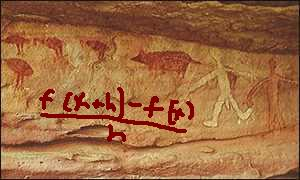
\includegraphics[width=0.382\textwidth]{pictures/cave}
  \end{center}
%\caption{You Know my Name}
\end{wrapfigure}
In früheren Aufgaben wurde die durchschnittliche Änderung einer Grösse berechnet; beispielsweise die durchschnittliche Geschwindigkeit einer Rakete, wenn man das Weg-Zeit-Diagramm kennt:
$$\bar{v}=\frac{\Delta s}{\Delta t}$$
wobei $\Delta s$ die Höhendifferenz und $\Delta t$ die Länge des zugehörigen Zeitintervalls ist.
Wie gross ist aber die Geschwindigkeit zu einem bestimmten Zeitpunkt, zum Beispiel $\unit[15]{s}$ nach dem Start? Einen ersten, noch ungenauen Näherungswert für die gesuchte Momentangeschwindigkeit liefert sicher die mittlere Geschwindigkeit im Zeitintervall $[15,20]$. Durch die Verkleinerung des Zeitintervalls kann die Genauigkeit verbessert werden.

\begin{uebenv}{freierfall}
Fällt ein Körper aus der Ruhelage im freien Fall $t$ Sekunden lang, so lässt sich der zurückgelegte Weg $s$ (in Meter) annähernd durch
$$s(t)=5t^2$$
berechnen.

Berechne die Durchschnittsgeschwindigkeiten in den Zeitintervallen $[3,3.5]$, $[3,3.2]$, $[3,3.1]$, $[3,3.05]$. Wie gross ist die Momentangeschwindigkeit nach genau drei Sekunden?
\end{uebenv}

Die entsprechende mathematische Formulierung lautet:
Die Momentangeschwindigkeit $v(t_0)$ zum Zeitpunkt $t_0$ ist der Grenzwert, gegen den die Durchschnittsgeschwindigkeit $\bar{v}$ im Zeitintervall $\Delta t=t_1-t_0$ strebt, wenn $t_1$ gegen $t_0$ geht ($\Delta t\rightarrow 0$). In Formeln:
$$v(t_0)=\lim_{t_1\rightarrow t_0}\bar{v}=\lim_{t_1\rightarrow t_0}\frac{\Delta s}{\Delta t}=\lim_{t_1\rightarrow t_0}\frac{s(t_1)-s(t_0)}{t_1-t_0}.$$
$s(t)$ bezeichne die bis zum Zeitpunkt $t$ erreichte Höhe.

\subsection{Das Konzept}
Eine beliebige Funktion $f$ sei im betrachteten Intervall $[a,b]$ stetig. Mit der Steigung der Sekante lässt sich das Änderungsverhalten der Funktion, d.h. die Steigung, an einer beliebigen, aber festgehaltenen Stelle $x_0\in[a,b]$ in einfacher Weise erklären. Will man nun das Änderungsverhalten der Funktion in $x_0$ exakt bestimmen, so ist dazu die Tangentensteigung im Punkt $P=(x_0|f(x_0))$ zu berechnen.

\begin{figure}
\begin{center}
\scalebox{1.25}{
\begin{tikzpicture}[line cap=round,line join=round,x=0.35cm,y=1cm]
\draw[->,color=black] (-2.53,0) -- (18.47,0);
\foreach \x in {-2,2,4,6,8,10,12,14,16,18}
\draw[shift={(\x,0)},color=black] (0pt,-2pt);
\draw[color=black] (17.99,0.05) node [anchor=south west] {$x$};
\draw[->,color=black] (0,-0.69) -- (0,5.12);
\foreach \y in {,1,2,3,4,5}
\draw[shift={(0,\y)},color=black] (2pt,0pt) -- (-2pt,0pt);
\draw[color=black] (0.14,4.87) node [anchor=west] {$y$};
\clip(-2.53,-0.69) rectangle (18.47,5.12);
\draw[line width=1pt, color=seagreen,smooth,samples=100,domain=-2.53:18.48] plot(\x,{0.02*\x^2+0.5});
\draw [domain=-2.53:18.47] plot(\x,{(-0.72--3.84*\x)/12});
\draw [domain=-2.53:18.47] plot(\x,{(--0.54--2.34*\x)/9});
\draw [domain=-2.53:18.47] plot(\x,{(--1.08--1.2*\x)/5.99});
\draw [dash pattern=on 4pt off 4pt] (14,4.42)-- (13.92,0);
\draw [dash pattern=on 4pt off 4pt] (2,0.58)-- (13.93,0.67);
\draw [dash pattern=on 4pt off 4pt] (2,0.58)-- (2,0);
\draw [line width=1pt,color=firebrick,domain=-2.53:18.47] plot(\x,{(--0.42--0.08*\x)/1});
\draw [color=firebrick](11.52,1.86) node[anchor=north west] {$t$};
\draw (7.53,0.63) node[anchor=north west] {$\Delta x$};
\draw (14.4,2.72) node[anchor=north west] {$\Delta f$};
\draw[color=darkblue] (12.8,4.86) node[anchor=north east] {$Q$};
\draw (1.5,-0.1) node[anchor=north west] {$x_0$};
\draw (13.2,-0.1) node[anchor=north west] {$x$};
\draw[color=seagreen] (-1.9,0.85) node {$f$};
\fill [color=black] (2,0.58) circle (1.5pt);
\draw[color=darkblue] (1.74,0.82) node {$P$};
\fill [color=darkblue] (14,4.42) circle (1.5pt);
\fill [color=darkblue] (11,2.92) circle (1.5pt);
\fill [color=darkblue] (7.99,1.78) circle (1.5pt);
\end{tikzpicture}
}
\caption{Übergang vom Differenzenquotienten zum Differenzialquotient}
\end{center}
\end{figure}

\begin{cdef}[Steigung]
Die Steigung der Tangente $t$ in $P$ wird als Steigung des Graphen in $P$, also als momentanes Änderungsverhalten der Funktion $f$ an einer Stelle $x_0$ bezeichnet.
\end{cdef}

Nachdem die Tangente im Punkt eines Graphen definiert ist, kann das Tangentenproblem rechnerisch formuliert werden. Es genügt, die Steigung der Tangente in $P$ zu ermitteln, da die Stelle $x_0$ bzw. der Punkt $P$ gegeben ist, womit die Lage der Tangente eindeutig bestimmt ist.

\pagebreak

\begin{cdef}[Differenzialquotient]
Die Steigung der Tangente erhält man für $\Delta x\rightarrow0$. Sie ist also
$$\lim_{x\rightarrow x_0}\frac{\Delta f(x_0)}{\Delta x}=\lim_{x\rightarrow x_0}\frac{f(x)-f(x_0)}{x-x_0}.$$
Falls dieser Grenzwert existiert, was ja keinesfalls sicher ist, da sowohl der Zähler als auch der Nenner gegen Null streben ($x_0$ ist eine Unbestimmtheitsstelle), nennt man diesen Grenzwert den Differenzialquotient von $f$ an der Stelle $x_0$.
\end{cdef}

Der Differenzialquotient ist der wichtigste Begriff der Differenzialrechnung. Mit ihm bewältigten Newton und Leibniz den Übergang von der antiken zur modernen Mathematik, da sie jetzt das momentane Änderungsverhalten einer Funktion bzw. die Steigung des Graphen an einer bestimmten Stelle $x_0$ rechnerisch untersuchen konnten.
Sowohl der Name Differenzialquotient als auch die Schreibweise $\frac{\mathrm{d}f(x_0)}{\mathrm{d}x}$ stammen von \textsc{Leibniz}.

Für die praktische Berechnung des Differenzialquotienten ersetzt man $x$ durch $x_0+h$ und lässt $h$ gegen $0$ streben. Der Differenzialquotient erhält dann die Form
$$\frac{\mathrm{d}}{\mathrm{d}x}f(x)|_{x=x_0}=\frac{\mathrm{d}f(x_0)}{\mathrm{d}x}=\lim_{h\rightarrow0}\frac{f(x_0+h)-f(x_0)}{h}.$$

\begin{uebenv}{aenderungsraten}
Vervollständige Tabelle \ref{tab:interpretation} auf Seite \pageref{tab:interpretation} mit weiteren Beispielen für lokale Änderungsraten.

\begin{table}[h]
\normalsize
\begin{center}
\begin{tabular}{|c|c|c|}
\hline
\rowcolor{Gray}\spaltenheight $x$ & $f(x)$ & $\frac{\mathrm{d}f(x)}{\mathrm{d}x}$ \spaltensep\hline
\rowcolor{lightyellow}\spaltenheight Abszisse & Ordinate & Graphensteigung \spaltensep\hline
\rowcolor{Gray}\spaltenheight Zeit & Ort & \spaltensep\hline
\rowcolor{lightyellow}\spaltenheight Zeit & & Beschleunigung \spaltensep\hline
\rowcolor{Gray}\spaltenheight Zeit & elektrische Ladung & \spaltensep\hline
\rowcolor{lightyellow}\spaltenheight  & Energie & Leistung \spaltensep\hline
\rowcolor{Gray}\spaltenheight  & chem. Konzentration & chem. Reaktionsgeschw.\spaltensep\hline
\rowcolor{lightyellow}\spaltenheight  Zeit & & Wachstumsgeschwindigkeit \spaltensep\hline
\rowcolor{Gray}\spaltenheight  Zeit & Geldwert & \spaltensep\hline
\end{tabular}
\end{center}
\caption{Interpretation des Differenzialquotienten}\label{tab:interpretation}
\end{table}
\end{uebenv}

\begin{uebenv}{differentialquotient}
Berechne
\marginnote{
\qrcode{
https://www.youtube.com/watch?v=z-42d5dtA_Q}
}
den Differenzialquotienten der Funktion $f$ an der Stelle $x_0$ und die Gleichung der Tangente im Punkt $P(x_0|f(x_0)$. Überprüfe dein Ergebnis mit einer Skizze.
\begin{enumerate}[a)]
\item $f(x)=x^2$ in $x_0=1$
\item $g(x)=-x^3$ in $x_0=-1$
\item $h(x)=x^{-1}$ in $x_0=0.25$
\end{enumerate}
\end{uebenv}

\begin{uebenv}{momentangeschw}
Berechne
\marginnote{
\qrcode{
https://www.youtube.com/watch?v=-KFROqbQkuA}
}
die Momentangeschwindigkeit zur Zeit $t=2$ für eine Bewegung mit

\begin{enumerate}[a)]
\item $s(t)=t^2+3t$
\item $s(t)=\sqrt{t}$
\end{enumerate}

wenn $t$ in Sekunden und $s(t)$ in Meter angegeben sind.
\end{uebenv}

\clearpage

\subsection{Notizen zu den Übungen}

\begin{lsg}{freierfall}
    Man hat für $\frac{\Delta s}{\Delta t}$ und die immer kleiner werden Intervalle $32.5$, $31$, $30.5$, $30.25$ Meter pro Sekunde. Vermutlich ist die Momentangeschwindigkeit nach 3 Sekunden $\unitfrac[30]{m}{s}$.
\end{lsg}
\begin{lsg}{aenderungsraten}
    \begin{table}[h]
\normalsize
\begin{center}
\begin{tabular}{|c|c|c|}
\hline
\rowcolor{Gray}\spaltenheight $x$ & $f(x)$ & $\frac{\mathrm{d}f(x)}{\mathrm{d}x}$ \spaltensep\hline
\rowcolor{lightyellow}\spaltenheight Abszisse & Ordinate & Graphensteigung \spaltensep\hline
\rowcolor{Gray}\spaltenheight Zeit & Ort & Geschwindigkeit\spaltensep\hline
\rowcolor{lightyellow}\spaltenheight Zeit & Geschwindigkeit & Beschleunigung \spaltensep\hline
\rowcolor{Gray}\spaltenheight Zeit & elektrische Ladung & Strom\spaltensep\hline
\rowcolor{lightyellow}\spaltenheight Zeit & Energie & Leistung \spaltensep\hline
\rowcolor{Gray}\spaltenheight Zeit & chem. Konzentration & chem. Reaktionsgeschw.\spaltensep\hline
\rowcolor{lightyellow}\spaltenheight  Zeit & Population & Wachstumsgeschwindigkeit \spaltensep\hline
\rowcolor{Gray}\spaltenheight  Zeit & Geldwert & Inflation/Deflation\spaltensep\hline
\end{tabular}
\end{center}
\caption{Interpretation des Differenzialquotienten}\label{tab:interpretation}
\end{table}
\end{lsg}
\begin{lsg}{differentialquotient}
    \begin{enumerate}[a)]
        \item
        \begin{align*}
        		\frac{\mathrm{d}f}{\mathrm{d}x} &= \lim_{h\to0}\frac{f(x_0+h)-f(x_0)}{h}=\lim_{h\to0}\frac{(x_0+h)^2-x_0^2}{h}=\lim_{h\to0}\frac{x_0^2+2x_0h+h^2-x_0^2}{h}\\
		&= \lim_{h\to0}\frac{2x_0h+h^2}{h}=\lim_{h\to0}2x_0+h=2x_0
	\end{align*}
	also $\frac{\mathrm{d}f(1)}{\mathrm{d}x}=2$
	
        \item
        \begin{align*}
        		\frac{\mathrm{d}g}{\mathrm{d}x} &= \lim_{h\to0}\frac{g(x_0+h)-g(x_0)}{h}=\lim_{h\to0}\frac{-(x_0+h)^3+x_0^3}{h}=\lim_{h\to0}\frac{-x_0^3-3x_0^2h-3x_0h^2-h^3+x_0^3}{h}\\
		&= \lim_{h\to0}\frac{-(x_0+h)^3+x_0^3}{h}=\lim_{h\to0}\frac{-3x_0^2h-3x_0h^2-h^3}{h}=\lim_{h\to0}-3x_0^2-3x_0h-h^2=-3x_0^2
        \end{align*}
	also $\frac{\mathrm{d}g(-1)}{\mathrm{d}x}=-3$
        \item
        \begin{align*}
        		\frac{\mathrm{d}h}{\mathrm{d}x} &= \lim_{h\to0}\frac{h(x_0+h)-h(x_0)}{h}=\lim_{h\to0}\frac{\frac{1}{x_0+h}-\frac{1}{x_0}}{h}=\lim_{h\to0}\frac{\frac{x_0}{x_0(x_0+h)}-\frac{x_0+h}{x_0(x_0+h)}}{h}\\
		&= \lim_{h\to0}\frac{\frac{-h}{x_0(x_0+h)}}{h}=\lim_{h\to0}\frac{-1}{x_0(x_0+h)}=-\frac{1}{x_0^2}
        \end{align*}
	somit $\frac{\mathrm{d}h(0.25)}{\mathrm{d}x}=-16$ 
    \end{enumerate}
\end{lsg}
\begin{lsg}{momentangeschw}
    \begin{enumerate}[a)]
        \item
        \begin{align*}
        		\frac{\mathrm{d}s}{\mathrm{d}t} &= \lim_{h\to0}\frac{s(t_0+h)-s(t_0)}{h}=\lim_{h\to0}\frac{(t_0+h)^2+3(t_0+h)-(t_0^2+3t_0)}{h}\\
		&= \lim_{h\to0}\frac{(t_0^2+2t_0h+h^2)+3(t_0+h)-(t_0^2+3t_0)}{h}=\lim_{h\to0}\frac{2t_0h+h^2+3h}{h}\\
		&= \lim_{h\to0}2t_0+h+3=2t_0+3
        \end{align*}
	und damit $v(3)=\unitfrac[9]{m}{s}$.
        \item
        \begin{align*}
        		\frac{\mathrm{d}s}{\mathrm{d}t} &= \lim_{h\to0}\frac{s(t_0+h)-s(t_0)}{h}=\lim_{h\to0}\frac{\sqrt{t_0+h}-\sqrt{t_0}}{h}=\lim_{h\to0}\frac{t_0+h-t_0}{h(\sqrt{t_0+h}+\sqrt{t_0})}\\
		&= \lim_{h\to0}\frac{h}{h(\sqrt{t_0+h}+\sqrt{t_0})}=\lim_{h\to0}\frac{1}{\sqrt{t_0+h}+\sqrt{t_0}}=\frac{1}{2\sqrt{t_0}}
        \end{align*}
	also $v(2)=\frac{1}{2\sqrt{2}}$ Meter pro Sekunde.
    \end{enumerate}
\end{lsg}

\clearpage

\section{Die Ableitung}
\subsection{Definition}

\begin{cdef}[Ableitung]
Existiert f\"ur jedes $x$ in einem Intervall der Grenzwert
$$\lim_{h\to0}\frac{f(x+h)-f(x)}{h}=\frac{\mathrm{d}f(x)}{\mathrm{d}x}$$
so kann damit eine neue Funktion $f'$ definiert werden. Bei dieser Funktion $f'$ wird jedem $x$ aus dem Intervall genau eine reelle Zahl, n\"amlich $\frac{\mathrm{d}f(x)}{\mathrm{d}x}$, zugeordnet.

Diese Funktion $f'$ --- die Symbolik stammt \"ubrigens von Leonard Euler --- nennt man Steigungsfunktion, weil jedem $x$ eine Steigung zugeordnet wird. Durch $f'$ wird das \"Anderungsverhalten der Ausgangsfunktion $f$ charakterisiert. $f'$ wird oft kurz als \emph{Ableitung} von $f$ bezeichnet.
\end{cdef}

\begin{uebenv}{steigungsfunktion}
Ermittle
\marginnote{
\qrcode{
https://www.youtube.com/watch?v=5RJYwSTO5w8}
}
die Steigungsfunktion (die Ableitung) $f'$ f\"ur
\begin{enumerate}[a)]
\item die Geraden mit den Gleichungen $f(x)=x$, $g(x)=2x-3$,
\item die Parabeln mit den Gleichungen $f(x)=x^2$, $g(x)=3x^2-2$,
\item die Hyperbeln mit der Gleichung $f(x)=\frac{2}{x}$
\item den Parabelast mit der Gleichung $f(x)=\sqrt{x}$,
\end{enumerate}
und die Steigungen in den Punkten $P(3|?)$ und $Q(-2|?)$.
\end{uebenv}

\begin{uebenv}{potenzregel}
Vervollst\"andige
\marginnote{
\qrcode{
https://www.youtube.com/watch?v=O722WzomYN4}
}
die Tabelle \ref{tab:abl} auf Seite \pageref{tab:abl}.

\begin{table}
\large
\begin{center}
\begin{tabular}{|c|c|}
\hline
\rule[-5mm]{0pt}{13mm}$f(x)=$ & $f'(x)=$\\ \hline
\rule[-5mm]{0pt}{15mm}$x^4$ & \\ \hline
\rule[-5mm]{0pt}{15mm}$x^3$ & \\ \hline
\rule[-5mm]{0pt}{15mm}$x^2$ & \\ \hline
\rule[-5mm]{0pt}{15mm}$x$ & \\ \hline
\rule[-5mm]{0pt}{15mm}$x^0$ & \\ \hline
\rule[-5mm]{0pt}{15mm}$\frac{1}{x}=x^{-1}$ & \\ \hline
\rule[-6mm]{0pt}{16mm}$\frac{1}{x^2}=x^{-2}$ & \\ \hline
\rule[-5mm]{0pt}{17mm}$\sqrt{x}=x^{\frac{1}{2}}$ & \\ \hline
\rule[-5mm]{0pt}{17mm}$\sqrt[3]{x}=x^{\frac{1}{3}}$ & \\ \hline
\rule[-5mm]{0pt}{17mm}$\sqrt{x^3}=x^{\frac{3}{2}}$ & \\ \hline
\end{tabular}
\caption{Wichtige Ableitungen}\label{tab:abl}
\end{center}
\end{table}
\end{uebenv}

\begin{lsg}{steigungsfunktion}
\begin{enumerate}[a)]
	\item $f'(x)=1$, $g'(x)=2$ und $f'(3)=1=f'(-2)$, $g'(3)=2=g'(-2)$
	\item $f'(x)=2x$, $g'(x)=6x$ und $f'(3)=6$, $f'(-2)=-4$, $g'(3)=18$, $g'(-2)=-12$
	\item $f'(x)=-\frac{2}{x^2}$ und $f'(3)=\frac{2}{9}$, $f'(-2)=-\frac{1}{2}$
	\item $f'(x)=\frac{1}{2\sqrt{x}}$ und $f'(3)=\frac{1}{2\sqrt{3}}$, $f'(-2)=\text{n.d.}$
\end{enumerate}
\end{lsg}

\begin{lsg}{potenzregel}
\def\mytabbottom{-2mm}
\def\mytabtop{6mm}
\begin{center}
\begin{tabular}{|c|c|}
\hline
\rule[\mytabbottom]{0pt}{\mytabtop}$f(x)=$ & $f'(x)=$\\ \hline
\rule[\mytabbottom]{0pt}{\mytabtop}$x^4$ & $4x^3$\\ \hline
\rule[\mytabbottom]{0pt}{\mytabtop}$x^3$ & $3x^2$\\ \hline
\rule[\mytabbottom]{0pt}{\mytabtop}$x^2$ & $2x$\\ \hline
\rule[\mytabbottom]{0pt}{\mytabtop}$x$ & $1$\\ \hline
\rule[\mytabbottom]{0pt}{\mytabtop}$x^0$ & $0$\\ \hline
\rule[\mytabbottom]{0pt}{\mytabtop}$\frac{1}{x}=x^{-1}$ & $-x^{-2}$\\ \hline\
\rule[\mytabbottom]{0pt}{\mytabtop}$\frac{1}{x^2}=x^{-2}$ & $-2x^{-3}$\\ \hline
\rule[\mytabbottom]{0pt}{\mytabtop}$\sqrt{x}=x^{\frac{1}{2}}$ & $\frac{1}{2}x^{-\frac{1}{2}}$\\ \hline
\rule[\mytabbottom]{0pt}{\mytabtop}$\sqrt[3]{x}=x^{\frac{1}{3}}$ & $\frac{1}{3}x^{-\frac{2}{3}}$\\ \hline
\rule[\mytabbottom]{0pt}{\mytabtop}$\sqrt{x^3}=x^{\frac{3}{2}}$ & $\frac{3}{2}x^\frac{1}{2}$\\ \hline
\end{tabular}
\end{center}
\end{lsg}

\clearpage

\subsection{Ableitungsregeln}

Die
\marginnote{
\qrcode{
https://www.youtube.com/watch?v=Jv0QEd45vqY}
}
vorherigen Aufgaben waren teilweise Beispiele f\"ur die folgenden allgemeinen Differenziations\-regeln.

Die beiden Funktionen $f$ und $g$ seien im betrachteten Intervall differenzierbar. Dann gelten:

\begin{itemize}
\item Eine konstante Funktion hat die Ableitung $0$.
$$(c)'=0$$
\item Ein konstanter Summand f\"allt bei der Differenziation weg.
$$(f(x)+c)'= f'(x)$$
\item Ein konstanter Faktor bleibt bei der Differenziation erhalten.
$$(cf(x))'=cf'(x)$$
\item Eine Summe von Funktionen darf man gliedweise differenzieren.
$$(f(x)+g(x))'=f'(x)+g'(x)$$
\end{itemize}

\begin{uebenv}{beweisableitungsregeln}
Beweise die vier Regeln mittels
$$F'(x)=\lim_{h\to0}\frac{F(x+h)-F(x)}{h}$$
\end{uebenv}

\begin{uebenv}{differenziere}
Differenziere die Funktionen

\begin{enumerate}[a)]
\item $\frac{1}{2}x^2-3x+2$
\item $5x^3+\frac{1}{3}x^2-2x-7$
\item $\frac{2}{x}-3x$
\item $\sqrt{x}-10x-(4x)^2$
\end{enumerate}
\end{uebenv}

\begin{uebenv}{glukose}
F\"ur
\marginnote{
\qrcode{
https://www.youtube.com/watch?v=CYY4jeCU_z4}
}
die Masse $M$ (in g) von Glukose bei einem Stoffwechselexperiment in Abh\"angigkeit der Zeit $t$ (in h) gilt:
$$M(t)=4.5-0.03t^2.$$
\begin{enumerate}
\item Wie gross ist die durchschnittliche \"Anderungsrate in den ersten beiden Stunden?
\item Berechne die momentane \"Anderungsrate f\"ur $t=0$ und $t=2$.
\end{enumerate}
\end{uebenv}

\begin{uebenv}{kugelvolumen}
Differenziere die Funktion $V$, deren Funktionswerte das Volumen einer Kugel mit dem Radius $r$ angeben. Was f\"allt auf?
\end{uebenv}

\begin{uebenv}{haengebruecke}
Die
\marginnote{
\qrcode{
https://www.youtube.com/watch?v=4nFIPeEDeMQ}
}
Tragseile einer H\"angebr\"ucke sind an den Pfeilern befestigt, die $\unit[250]{m}$ auseinander stehen, und h\"angen in Form einer Parabel, deren tiefster Punkt $\unit[50]{m}$ unter den Aufh\"angungspunkten liegt. Ermittle den Winkel zwischen Seil und Pfeiler.
\end{uebenv}

\begin{uebenv}{dewiesn}
Am
\marginnote{
\qrcode{
https://www.youtube.com/watch?v=Qsh0g0nuaoo}
}
Oktoberfest in M\"unchen sind in einem grossen Fass Bier anf\"anglich $\unit[2000]{Liter}$ Bier. Der Inhalt $V(t)$ des Fasses l\"asst sich in Abh\"angigkeit der Zeit $t$ in Minuten durch
$$V(t)=2000-\frac{5}{48}t^2+\frac{1}{3456}t^3$$
beschreiben.
\begin{enumerate}
\item Überprüfe, dass das Fass nach vier Stunden leer ist.
\item Wie viel Liter Bier fliessen genau 30 Minuten nach dem Anstich des Fasses in die Humpen?
\item Wann ist das Fest auf seinem \glqq H\"ohepunkt\grqq?
\end{enumerate}
\end{uebenv}

\begin{uebenv}{match}
Finde
\marginnote{
\qrcode{
https://www.youtube.com/watch?v=ZITSx3cx0L0}
}
zu den fünf Graphen a -- e in Abbildung \ref{derive} auf Seite \pageref{derive} jeweils die passende Ableitungsfunktion A -- E.

\begin{figure}
\begin{center}
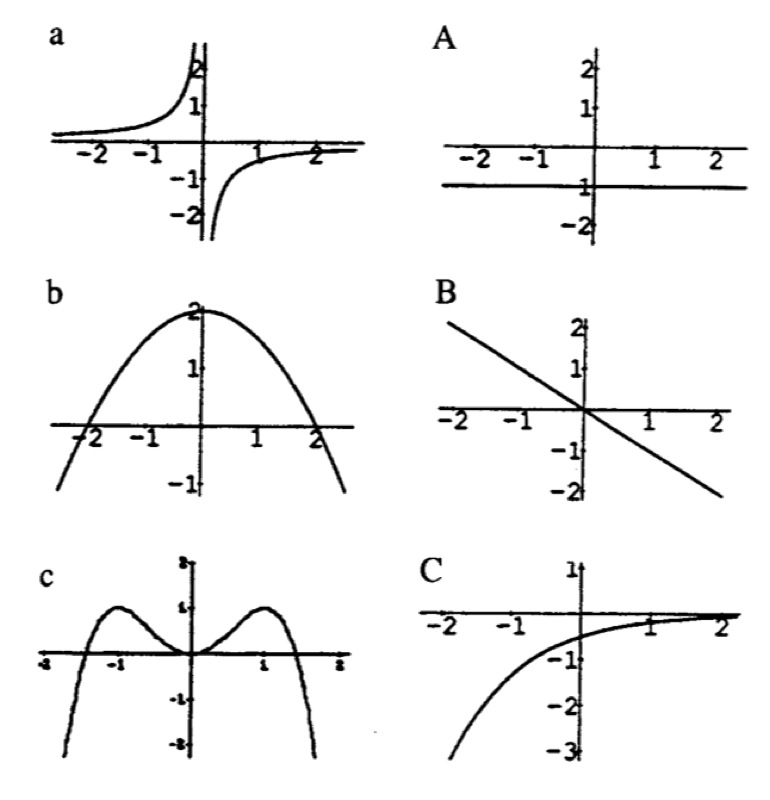
\includegraphics[width=0.45\textwidth,angle=0.6]{pictures/derivates1}
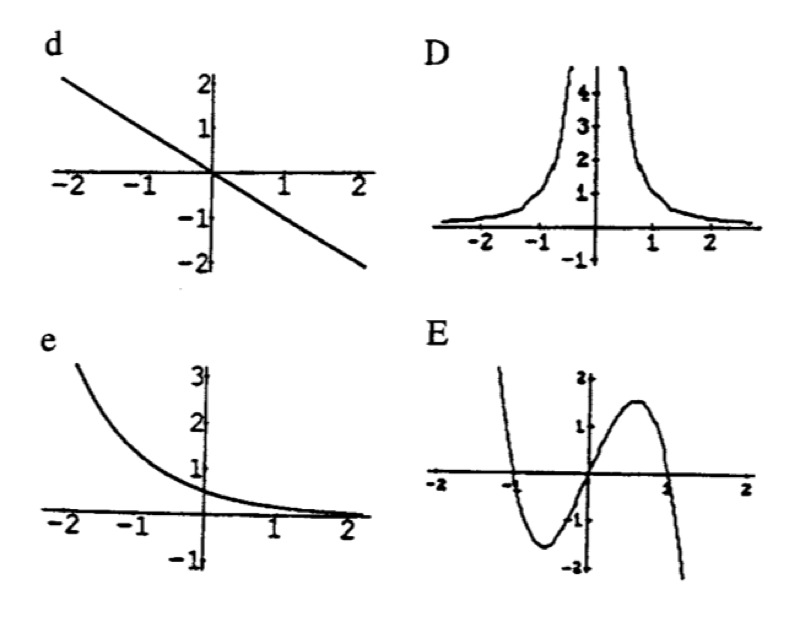
\includegraphics[width=0.45\textwidth,angle=0.6]{pictures/derivates2}
\end{center}
\caption{Graphen und ihre Ableitungsgraphen}\label{derive}
\end{figure}
\end{uebenv}

\clearpage

\subsection{Notizen zu den Übungen}

\begin{lsg}{beweisableitungsregeln}
    \begin{enumerate}[a)]
        \item $F(x)=c$ und daraus
        \begin{align*}
            \lim_{h\to0}\frac{F(x+h)-F(x)}{h} &= \lim_{h\to0}\frac{c-c}{h}=\lim_{h\to0}\frac{0}{h}=0
        \end{align*}
        \item $F(x)=f(x)+c$ und daraus
        \begin{align*}
            \lim_{h\to0}\frac{F(x+h)-F(x)}{h} &= \lim_{h\to0}\frac{f(x+h)+c-(f(x)+c)}{h}=\lim_{h\to0}\frac{f(x+h)-f(x)}{h}=f'(x)
        \end{align*}
        \item $F(x)=c\cdot f(x)$ und daraus
        \begin{align*}
            \lim_{h\to0}\frac{F(x+h)-F(x)}{h} &= \lim_{h\to0}\frac{c\cdot f(x+h)-(c\cdot f(x))}{h}=\lim_{h\to0}c\cdot\frac{f(x+h)-f(x)}{h}=c\cdot f'(x)
        \end{align*}
        \item $F(x)=f(x)+g(x)$ und daraus
        \begin{align*}
            \lim_{h\to0}\frac{F(x+h)-F(x)}{h} &= \lim_{h\to0}\frac{f(x+h)+g(x+h)-(f(x)+g(x))}{h}=\lim_{h\to0}\frac{f(x+h)-f(x)+g(x+h)-g(x)}{h}=\lim_{h\to0}\frac{f(x+h)-f(x)}{h}+\lim_{h\to0}\frac{g(x+h)-g(x)}{h}=f'(x)+g'(x)
        \end{align*}
    \end{enumerate}
\end{lsg}
\begin{lsg}{differenziere}
    \begin{enumerate}[a)]
        \item $x-3$
        \item $15x^2+\frac{2}{3}x-2$
        \item $-\frac{2}{x^2}-3$
        \item $-32x-10+\frac{1}{2\sqrt{x}}$
    \end{enumerate}
\end{lsg}
\begin{lsg}{glukose}
    \begin{enumerate}[a)]
        \item $\frac{\Delta M}{\Delta t}=\frac{M(2)-M(0)}{2}=\frac{4.38-4.5}{2}=-0.06$
        \item $M'(t)=-0.06t$ und somit $M'(0)=0$ bzw. $M'(2)=-0.12$
    \end{enumerate}
\end{lsg}
\begin{lsg}{kugelvolumen}
    Aus $V(r)=\frac{4}{3}\pi\cdot r^3$ folgt $V'(r)=4\pi r^2=O(r)$.
\end{lsg}
\begin{lsg}{haengebruecke}
    Ich nehme den Scheitelpunkt in den Ursprung. Damit werden die Aufhängepunkte $A_1(-125|50)$ und $a_2(125|50)$ und wir nehmen $f(x)=ax^2$ an. Es folgt $50=a\cdot125^2$ und sofort $a=\frac{50}{125^2}=0.0032$,
    $$f(x)=0.0032x^2.$$
    Der Winkel am Aufhängepunkt bezüglich der Horizontalen ist $f'(125)$. Es ist $f'(x)=0.0064$. Daraus folgt $f'(125)=0.8$ und $\alpha=\arctan(0.8)\approx38.7^\circ$. Also ist der Winkel zwischen Seil und Pfosten $180-90-38.7\approx51.3^\circ$.
\end{lsg}
\begin{lsg}{dewiesn}
    \begin{enumerate}[a)]
        \item $V(240)=2000-\frac{5}{48}\cdot240^2+\frac{1}{3456}\cdot240^3=0$.
        \item $V'(t)=-\frac{5}{24}t+\frac{1}{1152}t^2\quad\implies\quad V'(30)\approx-5.5$ Liter pro Minute
        \item Definieren wir den Höhepunkt, wenn am meisten Bier ausgeschenkt wird. Scheitelpunkt von $V'(t)$, dann findet die maximale Änderung des Fassinhalts statt. $t_s=-\frac{-\frac{5}{24}}{\frac{2}{1152}}=120$, also nach 2 Stunden.
    \end{enumerate}
\end{lsg}
\begin{lsg}{match}
    aD, bB, cE, dA, eC
\end{lsg}

\clearpage

\section{Weitere Ableitungsregeln}

Wollte man die Ableitung der Funktion
$$f(x)=\sin^3(x)\quad\text{oder}\quad g(x)=\frac{3x^2-7x+1}{x^3-2}$$
mittels dem Differenzialquotienten
$$\lim_{h\to0}\frac{f(x+h)-f(x)}{h}$$
berechnen, so wäre dies sicher ein mühsames Unterfangen. Mit einigen weiteren Differenziationsregeln lassen sich die nötigen Rechnungen erheblich vereinfachen.

\subsection{Produkt- und Quotientenregel}

Aus
$$f(x)=x^5=x^2\cdot x^3$$
und daraus
$$f'(x)=5x^4\neq 2x\cdot3x^2$$
erkennt man, dass die Ableitung eines Produkts nicht so einfach wie bei der Summe berechnet werden kann.

\begin{csatz}[Produktregel]
Sind
\marginnote{
\qrcode{
https://www.youtube.com/watch?v=KsMlJTZOaLA}
}
$f$ und $g$ an der Stelle $x$ differenzierbar, so ist auch ihr Produkt an dieser Stelle differenzierbar und der Differenzialquotient von $F(x)=f(x)\cdot g(x)$ lautet:
$$F'(x)=f'(x)\cdot g(x)+f(x)\cdot g'(x).$$
\end{csatz}

\begin{csatz}[Quotientenregel]
Sind $f$ und $g$ an der Stelle $x$ differenzierbar und $g(x)\neq0$, so ist auch ihr Quotient $f/g$ an dieser Stelle differenzierbar und der Differenzialquotient von $F(x)=f(x)/g(x)$ lautet:
$$F'(x)=\frac{f'(x)g(x)-f(x)g'(x)}{g(x)^2}.$$
\end{csatz}

\begin{proof}[Beweis Produktregel]
\begin{align*}
F'(x) &=\lim_{h\to0}\frac{F(x+h)-F(x)}{h}=\lim_{h\to0}\frac{f(x+h)g(x+h)-f(x)g(x)}{h}=\\
 &=\lim_{h\to0}f(x+h)\frac{g(x+h)-g(x)}{h}+\lim_{h\to0}\frac{f(x+h)-f(x)}{h}g(x)
\end{align*}

Da $f$ an der Stelle $x$ nach Voraussetzung differenzierbar ist, also dort sicher auch stetig, gilt $\lim_{h\to0}f(x+h)=f(x)$. Und daraus erhält man
$$F'(x)=f(x)\cdot g'(x)+f'(x)\cdot g(x)$$
\end{proof}

\begin{uebenv}{quotientenregel}
Beweise die Quotientenregel indem du
$$F(x)=\frac{f(x)}{g(x)}=f(x)\cdot\frac{1}{g(x)}$$
setzt und die Produktregel benutzt.
\end{uebenv}

\begin{uebenv}{tangente}
Berechne im Punkt $P(3|?)$ die Gleichung der Tangente an den Graphen der Funktion
$$f(x)=\frac{1-x}{1+x}.$$
In welchem Punkt hat der Graph eine zur ersten Winkelhalbierenden $g(x)=x$ parallele Tangente?
\end{uebenv}

\begin{uebenv}{uebenuebenueben}
Ermittle die Ableitung der folgenden Funktionen:

\begin{enumerate}[a)]
\item $f(x)=(x^2-1)(x^3+4)$
\item $f(x)=(x^3-2x+1)(2x^5+x^4-3x)$
\item $f(x)=\frac{x^4}{4}+3x^3+\frac{x^2}{2}+5x^{-3}$
\item $f(t)=(1+\frac{1}{t})(1-\frac{1}{t^2})$
\item $f(x)=\sqrt{7x}-5x+3x^{-1}+\frac{1}{8}x^8+\frac{1}{5}x^{-5}$
\item $f(t)=\frac{1}{t^2-1}$
\item $f(s)=\frac{4+s}{4-s}$
\item $f(x)=\frac{2x^2+1}{x+3}$
\item $f(t)=\frac{2t}{1+t^2}$
\item $f(x)=\frac{x^2-1}{x^2-4}$
\item $f(x)=\frac{x-5}{x^2-7x+12}$
\item $f(u)=\frac{u+1}{\sqrt{u}}$
\item $f(t)=\frac{1+\sqrt{t}}{1-\sqrt{t}}$
\end{enumerate}
\end{uebenv}

\subsection{Kettenregel}

Eine wichtige Regel für die Differenziation bezieht sich auf verschachtelte Funktionen:
$$F(x)=g(f(x)),$$
oder auch etwa in der Form
$$F(x)=g(u)\quad\text{mit}\quad u=f(x)$$
notiert. Zusammengesetzte Funktionen werden auch \definition{verkettete Funktionen} genannt.

\begin{bsp}
Die Funktion
$$F(x)=\sin(3x)$$
kann als Verkettung mit
$$g(u)=\sin(u)\quad\text{und}\quad f(x)=3x$$
interpretiert werden.
\end{bsp}

\begin{figure}[b]
\begin{center}
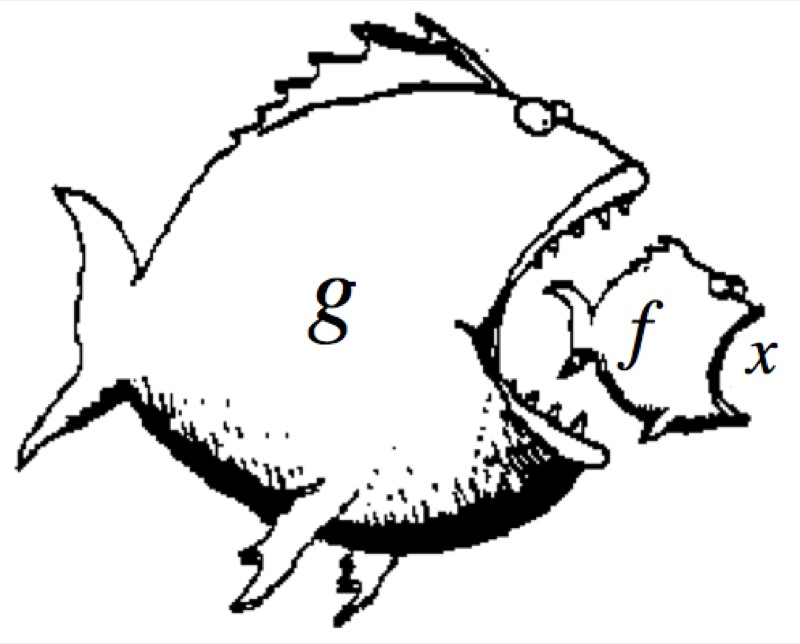
\includegraphics[width=0.15\textwidth]{pictures/verkettung}
\end{center}
\caption{Verkettung von Funktionen: hier $g(f(x))$}
\end{figure}

In der Mathematik ist die Schreibweise
$$(g\circ f)(x)=g(f(x))\quad\text{(sprich: g Ring f)}$$
üblich; insbesondere dann, wenn die Funktionen ohne Argument notiert werden. Beachte: $g\circ f$ bedeutet, dass zuerst $f$ und dann $g$ ausgeführt wird. Die Reihenfolge wird also von rechts nach links, wie im Arabischen, gelesen.

\begin{uebenv}{ring}
Ermittle die aus $f$ und $g$ zusammengesetzte Funktion
$$F(x)=(g\circ f)(x)$$
mit dem Funktionsterm $F(x)=g(f(x))$.
\begin{enumerate}
\item $f(x)=2x-1$, $g(x)=(x-3)^2+5$
\item $f(x)=x^2+1$, $g(x)=x^3+x^{-2}$
\end{enumerate}
\end{uebenv}

\begin{csatz}[Kettenregel]
\marginnote{
\qrcode{
https://www.youtube.com/watch?v=ZGOirKbLJUU}
}
$f$ an der Stelle $x$ und $g$ an der Stelle $f(x)$ differenzierbar, so ist auch ihre Verkettung $F=g\circ f$ mit $F(x)=g(f(x))$ in $x$ differenzierbar. Der Differenzialquotient von $F(x)=g(f(x))$ lautet:
$$F'(x)=g'(f(x))\cdot f'(x).$$
\end{csatz}

\begin{bem}
Man nennt $g$ die \definition{äussere}, $f$ die \definition{innere Funktion} und entsprechend $g'(f(x))$ die äussere und $f'(x)$ die innere Ableitung.
\end{bem}

\begin{bsp}
Für $F(x)=(10x^2-7x+3)^{100}$ ist $g(u)=u^{100}$ und $f(x)=10x^2-7x+3$, also $$F'(x)=100(10x^2-7x+3)^{99}\cdot(20x-7).$$

Für $f(x)=\sqrt{5x^7+3x^2+256}$ ist $g(u)=\sqrt{u}$ und $h(x)=5x^7+3x^2+256$, damit $$f'(x)=\frac{35x^6+6x}{2\sqrt{5x^7+3x^2+256}}.$$
\end{bsp}

\begin{proof}[Beweis Kettenregel]
Es seien $f,g$ differenzierbar und wir setzen $u=f(x)$ und $f(x+h)=f(x)+h*$. Aus der Stetigkeit von $f$ folgt: für $h\to0$ gilt auch $h*\to0$. So ergibt sich
\begin{align*}
F'(x)&=\lim_{h\to0}\frac{g(f(x+h))-g(f(x))}{h}=\\
&=\lim_{h\to0}\frac{g(u+h*)-g(u)}{h*}\cdot\frac{h*}{h}\\
&=\lim_{h\to0}\frac{g(u+h*)-g(u)}{h*}\cdot\frac{f(x+h)-f(x)}{h}\\
&=g'(u)\cdot f'(x) = g'(f(x))\cdot f'(x).
\end{align*}
\end{proof}

\begin{uebenv}{kettenregeluebenueben}
Ermittle die Ableitung der Funktionen:

\begin{enumerate}[a)]
    \item $f(x)=(4x^3-2x)^5$
    \item $f(x)=(x^2+x^{-1})^4$
    \item $f(x)=(x^2-5x+6)^{-3}$
    \item $f(t)=\sqrt{1+t^2}$
    \item $f(t)=\left(\frac{t^2+1}{t^2-1}\right)^2$
    \item $f(u)=\frac{1}{\sqrt{25-u^2}}$
\end{enumerate}
\end{uebenv}

\subsection{Ableitung der trigonometrischen Funktionen}

\begin{uebenv}{trigoableitungen}
Vermute
\marginnote{
\qrcode{
https://www.youtube.com/watch?v=2pExH_iwS9I}
}
aufgrund einer Zeichnung, welche Gestalt die Steigungsfunktion der Sinusfunktion hat.
\end{uebenv}

Mit den Additionstheoremen, die man leicht mit der Euleridentität ($\mathrm{e}^{i\varphi}=\cos(\varphi)+\mathrm{i}\sin(\varphi)$) nachweist, kann man Sinus und Cosinus überall differenzieren, wenn man die Ableitungen bei $0$ kennt:
$$\sin'(0 + a) = \sin'(0) \cos(a) + \cos'(0) \sin(a)$$
$$\cos'(0 + a) = \cos'(0) \cos(a) - \sin'(0) \sin(a).$$
Falls $\sin'(0)$ existiert, können wir mit der Kettenregel aus $\cos(x) = \sqrt{1-\sin^2(x)}$ folgern
$$\cos'(0)=\frac{-2\sin(0)\sin'(0)}{2\sqrt{1-\sin^2(0)}}=0.$$
Wir brauchen also nur
$$\lim_{h\to0}\frac{\sin(h)-\sin(0)}{h-0}=\lim_{h\to0}\frac{\sin(h)}{h}$$
Üblicherweise wird dazu benutzt (siehe auch unten)
$$\sin(h)\leq h\leq\tan(h)\longleftrightarrow\cos(h)\leq\frac{\sin(h)}{h}\leq1.$$
Wir sehen am Kreis unter anderem die Schranke $|\cos(\beta)-\cos(\alpha)|\leq|\beta-\alpha|$ und folgern $|\cos(0)-\cos(h)|\leq|0-h|$, also
$$\lim_{h\to0}\cos(h)=1.$$
Daher gilt auch
$$\sin'(0)=\lim_{h\to0}\frac{\sin(h)}{h}=1$$
und wir sind fertig.

\begin{csatz}[Ableitungen von $\sin$ und $\cos$]
    Nach den obigen Überlegungen gilt:
    $$\sin'(x)=\cos(x)\quad\text{und}\quad\cos'(x)=-\sin(x)$$
\end{csatz}

\begin{uebenv}{difftan}
Leite
\marginnote{
\qrcode{
https://www.youtube.com/watch?v=BH7eAN73sYM}
}
die Ableitungsfunktion von
$$f(x)=\tan(x)$$
her.
\end{uebenv}

\begin{uebenv}{weitereuebungen}
Bestimme die Ableitung:

\begin{enumerate}[a)]
\item $f(x)=\sin x+2\cos(x)$
\item $f(x)=x\sin x+\cos(x)$
\item $f(x)=\frac{1}{1+\cos(x)}$
\item $f(u)=\tan^2(u)$
\item $f(t)=\frac{t^2}{\sin(t)}$
\item $f(\varphi)=\frac{1}{2}a^2\sin(\varphi)$
\item $f(x)=\sin(4x)$
\item $f(t)=\sqrt{\cos(t)}$
\item $f(u)=\cos^2(u)$
\item $f(x)=\sin\frac{1}{x}$
\item $f(\varphi)=\cos(a\sqrt{\varphi})$
\item $f(t)=\tan^3(5t)$
\item $f(x)=x^2\cos(4x)$
\item $f(x)=x^{-2}\sin(4x)$
\end{enumerate}
\end{uebenv}

\begin{uebenv}{sincos}

\begin{enumerate}[a)]
\item Wo und unter welchem Winkel (Schnittwinkel der Tangenten im Schnittpunkt) schneiden sich die Graphen der Sinus- und der Cosinusfunktion im Intervall $[0,\frac{\pi}{2}]$?
\item Wo haben die Graphen im Intervall $[0,2\pi]$ die gleiche Steigung?
\end{enumerate}
\end{uebenv}

\begin{uebenv}{kolben}
Der 
\marginnote{
\qrcode{
https://www.youtube.com/watch?v=DEkaI0LpDBM}
}
Ort $x(t)$ eines Kolbens kann beschrieben werden durch
$$x(t)=\cos(20\pi t)+ \sqrt{25-\sin^2(20\pi t)},\quad t\text{ in }s$$

\begin{figure}[h!]
\begin{center}
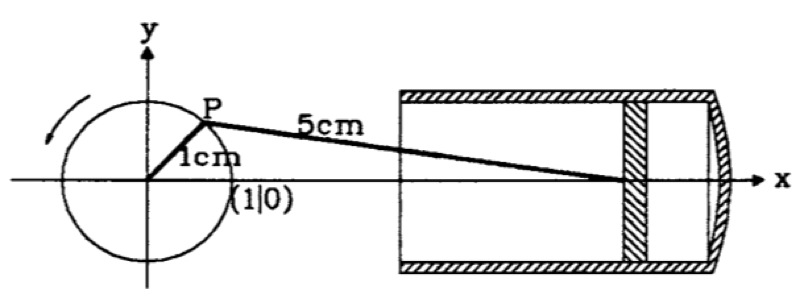
\includegraphics[width=8cm]{pictures/kolben}
\end{center}
\caption{Schema des Kolben}
\end{figure}

Wie schnell bewegt sich der Kolben zu den Zeiten $t=\frac{1}{40}$ und $t=\frac{1}{20}$ Sekunden?
\end{uebenv}

\subsection{Die Ableitung der Exponentialfunktion}

Um die Ableitung der Exponentialfunktion $\exp(x)=\mathrm{e}^x$ zu bestimmen, muss man den Grenzwert
$$\left(\mathrm{e}^x\right)'=\lim_{h\to0}\frac{\mathrm{e}^{x+h}-\mathrm{e}^x}{h}$$
untersuchen.

\begin{uebenv}{ableitungderexponentialfunktion}
Überzeuge dich davon, dass obiger Grenzwert gleich
$$\mathrm{e}^x\cdot\lim_{h\to0}\frac{\mathrm{e}^h-1}{h}$$
ist.
\end{uebenv}

Berechnet man Näherungswerte für den Grenzwert ($h\to0$) mit dem Taschenrechner, so drängt sich die Vermutung
$$\lim_{h\to0}\frac{\mathrm{e}^h-1}{h}=1$$
auf. Dies würde bedeuten, dass die Ableitung der $\mathrm{e}$-Funktion just wieder die $\mathrm{e}$-Funktion ist:
$$\left(\mathrm{e}^x\right)'\stackrel{?}{=}\mathrm{e}^x$$

Wir begnügen uns hier mit folgender Herleitung:
Für $h<1$ gilt
$$1+h\leq \mathrm{e}^h\leq\frac{1}{1-h}$$
Diese Ungleichungen können mit der Reihendefinition von $\mathrm{e}$ bzw. mit der geometrischen Reihe für $\frac{1}{1-h}$, falls $-1<h<1$, erklären.

\begin{center}
\begin{tikzpicture}[line cap=round,line join=round,>=triangle 45,x=1.5cm,y=1.1cm]
\draw[->,color=black] (-2.1,0) -- (2.2,0);
\foreach \x in {-2,-1,1,2}
\draw[shift={(\x,0)},color=black] (0pt,2pt) -- (0pt,-2pt);
\draw[color=black] (2,0.1) node [anchor=south west] {$x$};
\draw[->,color=black] (0,-0.5) -- (0,3.9);
\foreach \y in {,1,2,3}
\draw[shift={(0,\y)},color=black] (2pt,0pt) -- (-2pt,0pt);
\draw[color=black] (0.04,3.8) node [anchor=west] {$y$};
\clip(-2.04,-0.44) rectangle (2.12,3.91);
\draw[smooth,color=darkblue,samples=100,domain=-2.1:2.12] plot(\x,{1+\x});
\draw[smooth,color=seagreen,samples=100,domain=-2.1:2.12, thick] plot(\x,{2.71^(\x)});
\draw[smooth,color=darkblue,samples=100,domain=-2.01:0.93] plot(\x,{1/(1-(\x))});
\draw (-0.3,1.3) node[anchor=north west] {$1$};
\draw[color=darkblue] (1,1.5) node {\small$x+1$};
\draw[color=seagreen] (1.3,3) node {$\mathrm{e}^x$};
\draw[color=darkblue] (-1.4,0.7) node {$\frac{1}{1-x}$};
\end{tikzpicture}
\end{center}

also
$$h\leq \mathrm{e}^h-1\leq\frac{1}{1-h}-1=\frac{h}{1-h}$$
Es folgt für $h>0$
$$1\leq\frac{\mathrm{e}^h-1}{h}\leq\frac{1}{1-h},\text{ also }\lim_{h\downarrow0}\frac{\mathrm{e}^h-1}{h}=1$$
und für $h<0$
$$1\geq\frac{\mathrm{e}^h-1}{h}\geq\frac{1}{1-h},\text{ also }\lim_{h\uparrow0}\frac{\mathrm{e}^h-1}{h}=1$$
Insgesamt
$$\lim_{h\to0}\frac{\mathrm{e}^h-1}{h}=1$$

\begin{csatz}[Ableitung der $\mathrm{e}$-Funktion]
Die
\marginnote{
\qrcode{
https://www.youtube.com/watch?v=MkQ55zu9mEM}
}
Exponentialfunktion $\exp(x)=\mathrm{e}^x$ ist für alle $x\in\mathbb{R}$ differenzierbar, und es gilt
$$\left(\mathrm{e}^x\right)'=\mathrm{e}^x$$
\end{csatz}

\begin{bem}
Einen anderen Zugang hat man durch die Punkte:
\begin{itemize}
\item $\forall x\in\mathbb{R}\text{ ist }\mathrm{e}^x=\lim_{n\to\infty}\left(1+\frac{x}{n}\right)^n$
\item $<\left(1+\frac{x}{n}\right)^n>$ ist für $n>|x|$ monoton wachsend
\end{itemize}
also gilt $\left(1+\frac{x}{n}\right)^n\leq \mathrm{e}^x$.

Mit Hilfe der Bernoulli'schen Ungleichung erhält man dann die beiden Ungleichungen
$$1+x=1+n\frac{x}{n}\leq\left(1+\frac{x}{n}\right)^n\leq \mathrm{e}^x,$$
also $1+x\leq \mathrm{e}^x$ und, wenn man $x$ durch $-x$ ersetzt, $1-x\leq \mathrm{e}^{-x}=\frac{1}{\mathrm{e}^x}$.
Aus der zweiten Ungleichung ergibt sich für $1-x>0$ also
$\mathrm{e}^x\leq\frac{1}{1-x}.$
Damit gilt für $x<1$: 
$1+x\leq \mathrm{e}^x\leq\frac{1}{1-x}.$
\end{bem}

\subsection{Die Ableitung der Logarithmusfunktion}
Für
\marginnote{
\qrcode{
https://www.youtube.com/watch?v=HczWnwIKa4A}
}
die Herleitung erinnern wir uns daran, dass die Logarithmusfunktion $\ln(x)$ Inversfunktion der Exponentialfunktion $\mathrm{e}^x$ ist. Allgemein gilt für eine Funktion $f$ und ihre Inverse $f^{-1}$:
$$f(f^{-1}(x))=f^{-1}(f(x))=x.$$
Wenden wir diese Beziehung auf $\exp$ und $\ln$ an --- und berücksichtigen, dass $\ln$ nur für positive Argumente definiert ist --- haben wir
$$\mathrm{e}^{\ln(x)}=x$$
Beide Seiten der Gleichung abgeleitet ergibt:
$$\mathrm{e}^{\ln(x)}\cdot(\ln(x))'=1$$
und daraus folgt unmittelbar
$$(\ln(x))'=\frac{1}{x}.$$

\begin{csatz}[Ableitung des $\ln$]
Die
\marginnote{
\qrcode{
https://www.youtube.com/watch?v=soVDopFBghg}
}
Logarithmusfunktion $\ln(x)$ ist für alle $x\in\mathbb{R}^+$ differenzierbar und es gilt
$$(\ln(x))'=\frac{1}{x}.$$
\end{csatz}

\begin{uebenv}{weitereuebungen}
Ermittle die Definitionsmenge und die Ableitung der Funktion ($\mapsto$ bedeutet: \glqq wird zugeordnet\grqq)

\begin{enumerate}[a)]
\item $7\ln(x)$
\item $(\ln(x))^2$
\item $\ln(x-5)$
\item $\ln(\ln(x))$
\item $\sqrt{\ln(x)}$
\item $\ln(\sin(x))$
\item $3\mathrm{e}^{x}$
\item $\mathrm{e}^{3x}$
\item $6\mathrm{e}^{-5t+2}$
\item $\mathrm{e}^{2t^4-1}$
\item $\sqrt{t}\mathrm{e}^{\sqrt{t}}$
\item $\mathrm{e}^{-t^2}\ln(t)$
\end{enumerate}
\end{uebenv}

\clearpage

\subsection{Notizen zu den Übungen}

\begin{lsg}{quotientenregel}
    Betrachte
    \begin{align*}
        \left(\frac{f(x)}{g(x)}\right)' &= \left(f(x)\cdot\frac{1}{g(x)}\right)' = \left(f(x)\cdot[{g(x)}]^{-1}\right)'\\
        &= f'(x)\cdot[{g(x)}]^{-1}+f(x)\cdot(-[{g(x)}]^{-2}\cdot g'(x))
        = \frac{f'(x)}{[{g(x)}]^{-1}}+\frac{f(x)\cdot g'(x)}{-[{g(x)}]^{2}}\\
        &= \frac{f'(x)g(x)-f(x)g'(x)}{[{g(x)}]^{2}}
    \end{align*}
\end{lsg}
\begin{lsg}{tangente}
    Wir halten $\mathbb{D}=\mathbb{R}\setminus\{-1\}$ fest. Die Steigung ist $f'(x)=\left(\frac{1-x}{1+x}\right)=\frac{-(1+x)-(1-x)}{(1+x)^2}=\frac{-2}{(1+x)^2}$. An der Stelle $3$: $f'(3)=-\frac{1}{8}$ und damit als Ansatz für die Tangente $t(x)=-\frac{1}{8}x+q$. Ferner ist $f(3)=-\frac{1}{2}$, was wir in $t$ einsetzen:
    \begin{align*}
        t(3) &= -\frac{1}{2}\\
        -\frac{1}{8}\cdot3+q &= -\frac{1}{2}\\
        q &= -\frac{1}{8}
    \end{align*}
    Die Tangentengleichung lautet $t(x)=-\frac{1}{8}x-\frac{1}{8}$.
    
    Aus $g'(x)=1=\frac{-2}{(1+x)^2}$ folgt $x^2+2x+3=0$ mit Diskriminante $2^2-4\cdot3<0$. Daher beträgt die Steigung von $f$ an keiner Stelle $0$.
\end{lsg}
\begin{lsg}{uebenuebenueben}
    \begin{enumerate}[a)]
        \item $2x(x^3+4)+(x^2-1)\cdot3x^2$
        \item $(3x^2-2)(2x^5+x^4-3x)+(x^3-2x+1)(10x^4+4x^3-3)$
        \item $x^3+9x^2+x-15x^{-4}$
        \item $(-t^{-2})(1-\frac{1}{t^2})+(1+\frac{1}{t})\cdot t^{-3}$
        \item $\frac{\sqrt{7}}{2}x^{-\frac{1}{2}}-5-3x^{-2}+x^7+-x^{-6}$
        \item $\frac{-2t}{(t^2-1)^2}$
        \item $\frac{(4-s)-(4+s)(-1)}{(4-s)^2}$
        \item $\frac{4x(x+3)-(2x^2+1)}{(x+3)^2}$
        \item $\frac{2(1+t^2)-2t\cdot2t}{(1+t^2)^2}$
        \item $\frac{2x(x^2-4)-(x^2-1)\cdot 2x}{(x^2-4)^2}$
        \item $\frac{(x^2-7x+12)-(x-5)(2x-7)}{(x^2-7x+12)^2}$
        \item $\frac{\sqrt{u}-(u+1)\cdot\frac{1}{2}u^{-\frac{1}{2}}}{u}$
        \item $\frac{\frac{1}{2}t^{-\frac{1}{2}}(1-\sqrt{t}-(1+\sqrt{t})(-\frac{1}{2}t^{-\frac{1}{2}})}{(1-\sqrt{t})^2}$
    \end{enumerate}
\end{lsg}
\begin{lsg}{ring}
    \begin{enumerate}[a)]
        \item $g(f(x))=g(2x-1)=(2x-4)^2+5$
        \item $g(f(x))=g(x^2+1)=(x^2+1)^3+(x^2+1)^{-2}$
    \end{enumerate}
\end{lsg}
\begin{lsg}{kettenregeluebenueben}
    \begin{enumerate}[a)]
        \item $5(4x^3-2x)^4(12x^2-2)$
        \item $4(x^2+x^{-1})^3(2x-x^{-2}$
        \item $(-3)(x^2-5x+6)^{-4}(2x-5)$
        \item $\frac{1}{2}(1+t^2)^{-\frac{1}{2}}2t$
        \item $2\left(\frac{t^2+1}{t^2-1}\right)\left(\frac{2t(t^2-1)-(t^2+1)\cdot2t}{(t^2-1)^2}\right)$
        \item $-\frac{1}{2}(25-u^2)^{-\frac{3}{2}}(-2u)$
    \end{enumerate}
\end{lsg}
\begin{lsg}{trigoableitungen}
    Man zeichne die Graphen mit \geogebralink\ und vermutet $(\sin(x))'=\cos(x)$ und $(\cos(x))'=-\sin(x)$.
\end{lsg}
\begin{lsg}{difftan}
    Wir schreiben Tangens mit Sinus und Cosinus und leiten ab.
    \begin{align*}
        \tan'{x} &= \left(\frac{\sin(x)}{\cos(x)}\right)'=\frac{\cos(x)\cos(x)-\sin(x)(-\sin(x))}{\cos^2(x)}\\
        &= \frac{\cos^2(x)+\sin^2(x)}{\cos^2(x)} = \frac{1}{\cos^2(x)}
    \end{align*}
    Im letzten Schritt hätten wir auch den Bruch aufspalten können, um $\tan'(x)=1+\tan^2(x)$ zu erhalten.
\end{lsg}
\begin{lsg}{weitereuebungen}
\begin{enumerate}[a)]
        \item $\cos(x)-2\sin(x)$
        \item $\sin(x)+x\cos(x)-\sin(x)=x\cos(x)$
        \item $-(1+\cos(x))^{-2}(-\sin(x))$
        \item $2\tan(u)\cdot(1+\tan^2(u))$
        \item $\frac{2t\sin(t)-t^2\cos(t)}{\sin^2(t)}$
        \item $\frac{1}{2}(\cos(t))^{-\frac{1}{2}}\cdot(-\sin(t))$
        \item $2\cos(u)(-\sin(u))$
        \item $\cos(\frac{1}{x})(-x^{-2})$
        \item $-\sin(a\varphi)\cdot\frac{1}{2}\varphi^{-\frac{1}{2}}$
        \item $3\tan^2(5t)(1+\tan^2(5t))\cdot5$
        \item $2x\cos(4x)+x^2(-\sin(4x))\cdot4$
        \item $-2x^{-3}\sin(4x)+x^{-2}\cos(4x)\cdot4$
\end{enumerate}
\end{lsg}
\begin{lsg}{sincos}
    \begin{enumerate}[a)]
        \item $\sin(x)=\cos(x)\Leftrightarrow \frac{\sin(x)}{\cos(x)}=1\Leftrightarrow\tan(x)=1$ und damit $x=\frac{\pi}{4}\pm 2k\pi$ mit $k\in\mathbb{Z}$. Mit den Ableitungen $\cos(x)$ und $-\sin(x)$ berechnen wir die Steigung zu $\arccos(\frac{\pi}{4})=\frac{\sqrt{2}}{2}$ und $-\arcsin(\frac{\pi}{4})=-\frac{\sqrt{2}}{2}$. Wir berechnen $\arctan(\frac{\sqrt{2}}{2})\approx35.3^\circ$ und damit für den Zwischenwinkel $70.6^\circ$.
        \item Nun setzten wir $\cos(x)=-\sin(x)$ und erhalten $x=-\frac{\pi}{4}+2k\pi$ mit $k\in\mathbb{Z}$. Also hat man an der Stelle $x=\frac{7}{4}\pi$.
    \end{enumerate}
\end{lsg}
\begin{lsg}{kolben}
    Die Ableitung des Ortes nach der Zeit ist die Geschwindigkeit:
    $$\dot{x}=-\sin(20\pi t)\cdot20\pi+\frac{1}{2}(25-\sin^2(20\pi t))^{-\frac{1}{2}}\cdot(-2\sin(20\pi t))\cdot\cos(20\pi t)\cdot20\pi.$$
    Also folgt $v(\frac{1}{20})=0$ und $v(\frac{1}{40})=-20\pi$.
\end{lsg}
\begin{lsg}{ableitungderexponentialfunktion}
\begin{align*}
    \left(\mathrm{e}^x\right)' &= \lim_{h\to0}\frac{\mathrm{e}^{x+h}-\mathrm{e}^x}{h} = \lim_{h\to0}\frac{\mathrm{e}^{x}\cdot\mathrm{e}^h-\mathrm{e}^{x}}{h} = \lim_{h\to0}\frac{\mathrm{e}^{x}(\mathrm{e}^h-1)}{h}\\
    &= \mathrm{e}^{x}\cdot\lim_{h\to0}\frac{\mathrm{e}^h-1}{h}
\end{align*}
\end{lsg}
\begin{lsg}{weitereuebungen}
    \begin{enumerate}[a)]
        \item $7\cdot\frac{1}{x}$
        \item $2\ln(x)\cdot\frac{1}{x}$
        \item $\frac{1}{x-5}$
        \item $\frac{1}{\ln(x)}\cdot\frac{1}{x}$
        \item $\frac{1}{2}(\ln(x))^{-\frac{1}{2}}\cdot\frac{1}{x}$
        \item $\frac{1}{\sin(x)}\cdot\cos(x)$
        \item $3\mathrm{e}^x$
        \item $\mathrm{e}{3x}\cdot3$
        \item $6\mathrm{e}^{-5t+2}\cdot(-5)$
        \item $\mathrm{e}^{2t^4-1}\cdot(8t^3)$
        \item $\frac{1}{2}t^{-\frac{1}{2}}\cdot\mathrm{e}^{\sqrt{t}}+\sqrt{t}\cdot\mathrm{e}^{\sqrt{t}}\cdot\frac{1}{2}t^{-\frac{1}{2}}$
        \item $\mathrm{e}^{-t^2}\cdot(-2t)\ln(t)+\mathrm{e}^{-t^2}\cdot\frac{1}{t}$
    \end{enumerate}
\end{lsg}

\clearpage

\section{Graphenanalyse}

\subsection{Extrema}

\begin{cdef}[Extrema]
Der Punkt $(x_0|f(x_0))$ heisst \emph{relatives Minimum} oder Tiefpunkt, falls
$$f(x)>f(x_0)$$
für alle $x$ in einer hinreichend kleinen Umgebung von $x_0$.
\begin{center}
\definecolor{xdxdff}{rgb}{0.49,0.49,1}
\scalebox{0.9}{
\begin{tikzpicture}[line cap=round,line join=round,>=triangle 45,x=0.8cm,y=0.8cm]
\draw[->,color=black] (-0.48,0) -- (8.9,0);
\foreach \x in {,1,2,3,4,5,6,7,8}
\draw[shift={(\x,0)},color=black] (0pt,2pt) -- (0pt,-2pt);
\draw[color=black] (8.56,0.08) node [anchor=south west] {$x$};
\draw[->,color=black] (0,-0.86) -- (0,4.36);
\foreach \y in {,1,2,3,4}
\draw[shift={(0,\y)},color=black] (2pt,0pt) -- (-2pt,0pt);
\draw[color=black] (0.1,3.96) node [anchor=west] {$y$};
\clip(-0.48,-0.86) rectangle (8.9,4.36);
\draw[smooth,color=seagreen,samples=100,domain=0.3:7.5,thick] plot(\x,{0.1*(\x-5)^2+1.5});
\draw [dotted] (5,1.5)-- (5,0);
\draw (3.9,2.5) node[anchor=north west] {Minimalpunkt};
\draw (4.72,-0.14) node[anchor=north west] {$x_0$ (Extremalstelle)};
\draw (0.7,1) node[anchor=north west] {Minimum (Extremwert)};
\fill [color=firebrick] (5,1.5) circle (1.5pt);
\end{tikzpicture}
}
\end{center}
$(x_0|f(x_0))$ heisst \emph{relatives Maximum} oder Hochpunkt, falls
$$f(x)<f(x_0)$$
für alle $x$ in einer hinreichend kleinen Umgebung von $x_0$.
\begin{center}
\scalebox{0.9}{
\begin{tikzpicture}[line cap=round,line join=round,>=triangle 45,x=0.8cm,y=0.8cm]
\draw[->,color=black] (-0.48,0) -- (8.9,0);
\foreach \x in {,1,2,3,4,5,6,7,8}
\draw[shift={(\x,0)},color=black] (0pt,2pt) -- (0pt,-2pt);
\draw[color=black] (8.56,0.08) node [anchor=south west] {$x$};
\draw[->,color=black] (0,-0.86) -- (0,4.36);
\foreach \y in {,1,2,3,4}
\draw[shift={(0,\y)},color=black] (2pt,0pt) -- (-2pt,0pt);
\draw[color=black] (0.1,3.96) node [anchor=west] {$y$};
\clip(-0.48,-0.86) rectangle (8.9,4.36);
\draw[smooth,color=seagreen,samples=100,domain=0.4:6.0, thick] plot(\x,{0-(0.2)*(\x-4)^2+3});
\draw [dotted] (4,3)-- (4,0);
\draw (2.96,3.7) node[anchor=north west] {Maximalpunkt};
\draw (3.1,1.64) node[anchor=north west] {Maximum (Extremalwert)};
\draw (3.62,-0.3) node[anchor=north west] {$x_0$ (Extremalstelle)};
\fill [color=firebrick] (4,3) circle (1.5pt);
\end{tikzpicture}
}
\end{center}
\end{cdef}

\clearpage

Wie man diese Punkte rechnerisch findet, beschreiben die folgenden beiden Sätze.
\begin{csatz}[Extremum]
Hat
\marginnote{
\qrcode{
https://www.youtube.com/watch?v=VloOTGZ8SGQ}
}
die Funktion $f$ im Punkt $x_0$ ein relatives Minimum oder Maximum, dann gilt
$$f'(x_0)=0.$$
\end{csatz}
Beachte, dass diese Bedingung für eine Extremalstelle notwendig, aber nicht hinreichend, ist. Um zu entscheiden, ob sich im Punkt $x_0$ ein Minimum oder Maximum befindet, hilft der folgende

\begin{csatz}[Krümmung]
Ist $f''(x_0)>0$, dann ist der Graph von $f$ dort linksgekrümmt. Ist $f''(x_0)<0$, dann ist der Graph von $f$ dort rechtsgekrümmt.
\end{csatz}

Zusammengefasst heisst dies, wenn $f$ ein Minimum in $x_0$ hat, dann ist dort $f'(x_0)=0$ und $f''(x_0)>0$, und wenn $f$ ein Maximum in $x_0$ hat, dass $f'(x_0)=0$ und $f''(x_0)<0$ ist.

\subsection{Wendepunkte}

Das letzte Resultat wirft die Frage auf, wie ein Punkt $x_0$ von $f$ interpretiert werden soll, falls dort $f'(x_0)=0$ und $f''(x_0)=0$ ist. Wenn wir uns daran erinnern, dass die erste Ableitung einer Funktion die Steigung und die zweite Ableitung die Krümmung in einer hinreichend kleinen Umgebung von $x_0$ angibt, dann bedeutet $f''(x_0)=0$ also, dass dort der Graph von $f$ keine Krümmung besitzt.

\begin{cdef}[Terrassenpunkt]
Man nennt einen Punkt $(x_0|f(x_0))$ Terrassenpunkt von $f$, falls $f'(x_0)=0$, $f''(x_0)=0$ und $f'''(x_0)\neq0$ gilt.
\end{cdef}

\begin{center}
\begin{tikzpicture}[line cap=round,line join=round,>=triangle 45,x=0.8cm,y=0.8cm]
\draw[->,color=black] (-0.48,0) -- (8.12,0);
\foreach \x in {,1,2,3,4,5,6,7}
\draw[shift={(\x,0)},color=black] (0pt,2pt) -- (0pt,-2pt);
\draw[color=black] (7.78,0.08) node [anchor=south west] {$x$};
\draw[->,color=black] (0,-0.72) -- (0,4.36);
\foreach \y in {,1,2,3,4}
\draw[shift={(0,\y)},color=black] (2pt,0pt) -- (-2pt,0pt);
\draw[color=black] (0.1,3.96) node [anchor=west] {$y$};
\clip(-0.48,-0.72) rectangle (8.12,4.36);
\draw[smooth,color=seagreen, thick, samples=100,domain=0.3:7.0] plot(\x,{0.1*(\x-3.5)^3+2});
\draw [dash pattern=on 3pt off 3pt] (0.46,2)-- (6.6,2);
\draw [dotted] (3.5,2)-- (3.5,0);
\draw (3.2,0) node[anchor=north west] {$x_0$};
\draw (1.4,2.9) node[anchor=north west] {Terrassenpunkt};
\draw[color=seagreen] (0.8,-0.48) node {$f$};
\fill [color=firebrick] (3.5,2) circle (1.5pt);
\end{tikzpicture}
\end{center}

Schliesslich will ich noch einen letzten Begriff zur Kurvendiskussion einführen, den sogenannten \definition{Wendepunkt}. Man spricht dann von einem Wendepunkt von $f$ an der Stelle $x_0$, wenn $f''(x_0)=0$ und $f'''(x_0)\neq0$.
\begin{bem}
Ein Terrassenpunkt ist also ein spezieller Wendepunkt, nämlich ein Wendepunkt mit Horizontaltangente.
\end{bem}

\subsection{Überblick}
\marginnote{
\qrcode{
https://www.youtube.com/watch?v=X6RepNNUTLw}
}
\begin{itemize}
\item Hat $f$ an der Stelle $x_0$ ein Extremum, dann gilt
$$f'(x_0)=0$$
\item Hat $f$ an der Stelle $x_0$ einen Wendepunkt, dann gilt
$$f''(x_0)=0$$
\item Gilt $f'(x_0)=0$ und $f''(x_0)\neq0$, dann hat $f$ an der Stelle $x_0$ ein Extremum, und zwar
\begin{itemize}
\item ein Maximum, falls
$$f''(x_0)<0$$
\item ein Minimum, falls
$$f''(x_0)>0$$
\end{itemize}
\item Gilt $f''(x_0)=0$ und $f'''(x_0)\neq0$, dann hat $f$ einen Wendepunkt in $x_0$.
\end{itemize}

\begin{bem}
Die Umkehrung dieser Sätze gilt nicht.
\end{bem}

\begin{uebenv}{gegenbsp}
Überprüfe obige Aussage anhand einfacher Gegenbeispiele. Betrachte
$$f(x)=x^3\quad\text{und}\quad g(x)=x^4$$
in $x_0=0$.
\end{uebenv}

\begin{uebenv}{quadrfkt}
 Zeige, dass eine beliebige quadratische Funktion keinen Wendepunkt hat.
 \end{uebenv}
 
 \begin{uebenv}{polynomfktn}
 Bestimme die Nullstellen, Extrema und Wendestellen der Funktion
 $$f(x) = x^3-2x^2-5x+6.$$
 Zeige zuerst, dass bei $x=1$ eine Nullstelle ist und wende anschliessend Polynomdivision an, um die restlichen zu finden.
 \end{uebenv}

\begin{uebenv}{ganzrationalefkt}
Gib dir eine ganzrationale Funktion vor (z.B. $f(x)=4x^3-3x+1$) und untersuche diese nach Nullstellen, Extrema und Wendestellen. Überprüfe deine Berechnungen z.B. mit GeoGebra.
\end{uebenv}

\begin{uebenv}{sinanalysiert}
Zeichne die Sinusfunktion
$$f(x) = \sin{(x)}$$
im Intervall $[-4\pi,4\pi]$. Gib danach für $f$ Nullstellen, Symmetrie, Extrema und Wendestellen auf dem Definitionsbereich $\mathbb{D}=\mathbb{R}$ an. Zeichne mit einer andern Farbe ins gleiche Koordinatensystem die erste und zweite Ableitung von $f$ ein.
\end{uebenv}

\begin{uebenv}{glockenkurve}
Die
\marginnote{
\qrcode{
https://www.youtube.com/watch?v=rfXO1n9Av3I}
}
Funktion
$$g(x)=\mathrm{e}^{-x^2}$$
spielt in der Wahrscheinlichkeitsrechnung und Statistik eine beherrschende Rolle im Zusammenhang mit der Normal- oder Gauss'schen Verteilung.
\begin{enumerate}[a)]
\item Definitions- und Wertemenge,
\item Überprüfe, dass $g$ symmetrisch zur $y$-Achse ist.
\item $\lim_{x\to\pm\infty}f(x)$
\item Extremwerte
\item Wendepunkte des Graphen
\item Skizziere den glockenförmigen Graphen von $f$ mit den Informationen aus dieser Übung.
\end{enumerate}
\end{uebenv}

\clearpage

\subsection{Notizen zu den Übungen}

\begin{lsg}{gegenbsp}
    \begin{enumerate}[a)]
        \item Für $f(x)=x^3$ ist $f'(x)=3x^2$, $f''(x)=6x$ und $f'''(x)=6$. Aber $f$ hat in $x=0$ keine Extremalstelle, dafür aber eine Wendestelle; genauer eine Terrassenpunkt.
        \item Aus $g(x)=x^4$ folgt $g'(x)=4x^3$, $g''(x)=12x^2$, $g'''(x)=24x$ und $g''''(x)=12$. $g$ hat keine Wendestelle, aber ein Extremum.
    \end{enumerate}
\end{lsg}
 \begin{lsg}{quadrfkt}
     Sei $f(x)=ax^2+bx+c$ beliebig mit $a\neq0$. Es ist $f'(x)=2ax+b$, $f''(x)=2a$ und $f'''(x)=0$, also kann $f$ keinen Wendepunkt haben.
 \end{lsg}
 \begin{lsg}{polynomfktn}
     Es ist $f(1)=1^3-2\cdot1^2-5\cdot1+6=0$. Mit Polynomdivision finden wir
     \begin{align*}
         &(x^3-2x^2-5x+6) \div (x-1) = x^2-x-6\\
         &\underline{-(x^3-x^2)}\\
         &-x^2-5x+6\\
         &\underline{-(x^2+x)}\\
         &-6x+6\\
         &\underline{-(-6x+6)}\\
         &0
     \end{align*}
     Es folgt $x^2-x-6=(x-3)(x+2)=0$ und also $x_1=3$, $x_2=-2$. Wir haben alle Nullstellen. Für die Extrema brauchen wir erst $f'(x)\stackrel{!}{=}0\Leftrightarrow 3x^2-4x-5=0$, also $x=\frac{4\pm\sqrt{4^2-4\cdot3\cdot(-5)}}{6}=\frac{4\pm\sqrt{76}}{6}=\frac{4\pm2\sqrt{19}}{6}=\frac{2\pm\sqrt{19}}{3}$. Die Wendestellen berechnen wir zu $f''(x)=6x-4\stackrel{!}{=}0$, also $x=\frac{2}{3}$; $f'''(x)=6$. Man kann die Extremwerte noch klassifizieren.
 \end{lsg}
\begin{lsg}{ganzrationalefkt}
    Es ist $f(-1)=-4+3+1=0$, also ist $x_1=-1$ Nullstelle. $(4x^3-3x+1)\div(x+1)=4x^2-4x+1=0$ und es folgt $x_{2,3}=\frac{4\pm\sqrt{16-16}}{8}=\frac{1}{2}$. Extremwerte $f'(x)=12x^2-2\stackrel{!}{=}0\Leftrightarrow x=\pm\frac{1}{6}$, $f''(x)=24x$. Wendestelle bei $0$. Man kann die Extremwerte noch klassifizieren.
\end{lsg}
\begin{lsg}{sinanalysiert}
Nullstellen sind bei $\sin(x)=0$ und es folgt $x=k\pi$ mit $k\in\mathbb{Z}$. Extrema bei $\cos(x)=0\Rightarrow{}x=\frac{\pi}{2}+k\mathbb{Z}$ und Wendestellen bei $x=k\pi$ mit $k\in\mathbb{Z}$.

\begin{center}
    \begin{tikzpicture}
    \begin{axis}[
        axis lines = middle,
        xlabel = $x$,
        ylabel = $y$,
        legend pos = outer north east,
        grid = major,
        width = 11cm,
        height = 5cm,
        xtick={-3*pi,-2*pi, -pi, 0, pi, 2*pi,3*pi},
        xticklabels={$-3\pi$,$-2\pi$, $-\pi$, $0$, $\pi$, $2\pi$,$3\pi$},
        ytick={-1, 0, 1}
    ]
    \addplot[domain=-4*pi:4*pi, samples=100, darkblue, thick] {sin(deg(x))};
    \addlegendentry{$f(x)=\sin(x)$}
    \addplot[domain=-4*pi:4*pi, samples=100, firebrick, thick] {cos(deg(x))};
    \addlegendentry{$f'(x)=\cos(x)$}
    \addplot[domain=-4*pi:4*pi, samples=100, seagreen, thick] {-sin(deg(x))};
    \addlegendentry{$f''(x)=-\sin(x)$}
    \end{axis}
\end{tikzpicture}
\end{center}
\end{lsg}
\begin{lsg}{glockenkurve}
    \begin{enumerate}[a)]
        \item $\mathbb{D}=\mathbb{R}$, $\mathbb{W}=(0,1]$
        \item $g(-x)=\mathrm{e}^{-(-x)^2}=\mathrm{e}^{-x^2}=g(x)$, also symmetrisch zur $x$-Achse
        \item $g'(x)=0$ ist notwendig. $g'(x)=\mathrm{e}^{-x^2}\cdot(-2x)=0\Leftrightarrow x=0$, da $\mathrm{e}^{-x^2}>0\quad\forall x\in\mathbb{R}$. Betrachten wir noch $g''(x)=\mathrm{e}^{-x^2}\cdot(-2x)\cdot(-2x)+\mathrm{e}^{-x^2}\cdot(-2)=2\mathrm{e}^{-x^2}(2x^2-1)$ und somit $g''(0)=2\mathrm{e}^{0}(-1)=-2<0$ impliziert ein Maximum bei $x=0$.
        \item Für Wendestellen müssen wir $g''(x)=2\mathrm{e}^{-x^2}(2x^2-1)\Leftrightarrow x=\pm\frac{\sqrt{2}}{2}$ lösen, done.
        \item Der Graph sieht vielleicht so aus:
        
        \begin{center}
    \begin{tikzpicture}
    \begin{axis}[
        axis lines = middle,
        xlabel = $x$,
        ylabel = $y$,
        ymax = 1.3,
        legend pos = outer north east,
        grid = major,
        width = 11cm,
        height = 5cm,
        xtick={-3,-2,-1,0,1,2,3},
        xticklabels={-3,-2,-1,0,1,2,3},
        ytick={0, 0.5, 1}
    ]
    \addplot[domain=-4:4, samples=100, seagreen, very thick] {exp(-x^2)};
    \end{axis}
\end{tikzpicture}
\end{center}
    \end{enumerate}
\end{lsg}

\clearpage

\section{Extremwertaufgaben}

\begin{wrapfigure}{r}{0.382\textwidth}
\vspace{-22pt}
  \begin{center}
    
\includegraphics[width=0.382\textwidth]{pictures/can}
  \end{center}
%\caption{You Know my Name}
\vspace{-10pt}
\end{wrapfigure}
Man begegnet in unserer Umwelt sehr oft gewissen Grössen, die entweder zu minimieren (Kosten, Zeiten, Kraftaufwand,\dots) oder zu maximieren (Gewinne, Ausnutzung, Nutzeffekt,\dots) sind. Handelt es sich dabei um mehrere Variablen, die durch lineare Ungleichungen miteinander verbunden sind, so konnten diese Aufgaben mathematisch mit der linearen Optimierung gelöst werden. Im folgenden lässt sich der reale Zusammenhang durch eine differenzierbare Funktion mit nur einer Variablen beschreiben. Die Differenzialrechnung liefert dann mit ihren Methoden der Extremwertermittlung die Lösung des gestellten Problems.

\begin{bem}
Bei manchen Problemstellungen können \definition{Randextrema} vorkommen: Mit den Bezeichnungen aus Abbildung \ref{randextrem} auf Seite \pageref{randextrem} erreicht im Punkte $R$ die Funktion ihr globales Maximum (Randextremum). Im Punkt $Q$ erreicht sie ein lokales Maximum, während sie in $P$ sowohl ein globales als auch ein lokales Minimum erreicht.

\begin{figure}
\begin{center}
\scalebox{1.2}{
\begin{tikzpicture}[line cap=round,line join=round,x=0.7cm,y=0.7cm]
\draw[->,color=black] (-0.56,0) -- (9.07,0);
\foreach \x in {,2,4,6,8}
\draw[shift={(\x,0)},color=black] (0pt,2pt) -- (0pt,-2pt);
\draw[color=black] (8.73,0.08) node [anchor=south west] {$x$};
\draw[->,color=black] (0,-0.88) -- (0,4.36);
\foreach \y in {,2,4}
\draw[shift={(0,\y)},color=black] (2pt,0pt) -- (-2pt,0pt);
\draw[color=black] (0.1,3.95) node [anchor=west] {$y$};
\clip(-0.56,-0.88) rectangle (9.07,4.36);
\draw[smooth,samples=100,domain=0.2:8.0] plot(\x,{0-(0.03)*(\x-5)^3+0.3*\x});
\draw [dotted] (0.44,2.98)-- (0.44,0.02);
\draw [dotted] (7.81,1.68)-- (7.81,0);
\draw (0.2,0.05) node[anchor=north west] {$a$};
\draw (7.6,0.05) node[anchor=north west] {$b$};
\fill [color=darkblue] (0.44,2.98) circle (1.5pt);
\draw[color=darkblue] (0.6,3.4) node {$R$};
\fill [color=firebrick] (3.17,1.13) circle (1.5pt);
\draw[color=firebrick] (3.4,1.5) node {$P$};
\fill [color=darkblue] (6.83,1.87) circle (1.5pt);
\draw[color=darkblue] (6.99,2.2) node {$Q$};
\end{tikzpicture}
}
\end{center}
\caption{Randextremwert}\label{randextrem}
\end{figure}
\end{bem}

\begin{uebenv}{zerlegen}
Zerlege die Zahl 144 so in zwei Summanden, dass
\begin{enumerate}[a)]
\item ihr Produkt möglichst gross,
\item die Summe ihrer Quadrate möglichst klein wird.
\end{enumerate}
\end{uebenv}

\begin{lsg}{zerlegen}
    \begin{enumerate}[a)]
        \item Die beiden Summanden sind $x$ und $y=144-x$. Das Produkt ist somit $xy=x(144-x)=-x^2+144x$. Das Maximum ist der Scheitelpunkt $x_S=-\frac{144}{-2}=72$ und somit $y=72$. Das kriegt man auch über $(-x^2+144x)'=-2x+144=0$.
        \item Dazu untersuchen wir die Funktion $g(x)=x^2+(144-x)^2=2x^2-288x+144^2$ und leiten ab: $g'(x)=4x-288=0\Leftrightarrow x=72$, also auch $y=72$.
    \end{enumerate}
\end{lsg}

\begin{uebenv}{parabelloesen}
Zeichne in einem Koordinatensystem die Parabel mit der Gleichung
$$f(x) = 6 - \frac{x^2}{4}$$
Dem Abschnitt der Parabel, der oberhalb der $x$-Achse liegt, ist ein Rechteck mit mög\-lichst grossem
\begin{enumerate}[a)]
\item Inhalt,
\item Umfang
\end{enumerate}
einzubeschreiben.
\end{uebenv}

\begin{lsg}{parabelloesen}
        \begin{center}
    \begin{tikzpicture}
    \begin{axis}[
        axis lines = middle,
        xlabel = $x$,
        ylabel = $y$,
        ymax=7.5,
        legend pos = outer north east,
        grid = major,
        width = 11cm,
        height = 5cm,
        xlabel style={at={(axis description cs:1,0.2)}}
    ]
    \addplot[domain=-5.5:5.5, samples=100, seagreen, very thick] {6-0.25*x^2};
    %% Draw the inscribed rectangle with transparent and lightly hatched fill
    \addplot[firebrick, thick, fill=red, fill opacity=0.25, pattern=north east lines] coordinates {(-3.5, 0) (3.5, 0) (3.5, 6 - 0.25*3.5^2) (-3.5, 6 - 0.25*3.5^2) (-3.5, 0)};
    
    % Draw a red point at the left upper corner of the rectangle
    \addplot[only marks, mark=*, mark options={firebrick}] coordinates {(3.5, 6 - 0.25*3.5^2)} node[anchor=south west] {$(x|f(x))$};
    \end{axis}
\end{tikzpicture}
\end{center}
    \begin{enumerate}[a)]
        \item Der Inhalt ist $A(x)=xy=x(6-0.25x^2)=-0.25x^3+6x$. Maximal wird er bei $A'(x)=-0.75x^2+6=0$, also $x=\pm2\sqrt{2}$. Damit ist $A(2\sqrt{2})=8\sqrt{2}$.
        \item $U(x)=2x\cdot2f(x)=4x(6-0.25x^2)=-x^3+24x$. Somit $U'(x)=-3x^2+24$, also $x=2\sqrt{2}$.
    \end{enumerate}
\end{lsg}

\begin{uebenv}{buechse}
Eine
\marginnote{
\qrcode{
https://www.youtube.com/watch?v=6kFezQk7R-0}
}
kreiszylinderförmige Büchse hat den Inhalt $\unit[1]{l}$. Welche Abmessungen hat diese Büchse, wenn ihre Oberfläche, bestehend aus Mantel und Grundflächen, minimal werden soll?
\end{uebenv}

\begin{lsg}{buechse}
    $O=2\pi r^2+2\pi rh$ und $V=\pi r^2h$. Es folgt $h=\frac{V}{\pi r^2}$ und eingesetzt $O(r)=2\pi r^2+2\pi r\cdot\frac{V}{\pi r^2}=2\pi r^2+\frac{2V}{r}$.
    Daher $4\pi r-\frac{2V}{r^2}\stackrel{!}{=}0$ und daraus
    
    \begin{align*}
        4\pi r &= \frac{2V}{r^2}\\
        r^3 &= \frac{V}{2\pi}\\
        r &= \sqrt[3]{\frac{V}{2\pi}}
    \end{align*}
    
    Das ergibt für einen Liter Inhalt $r\approx\unit[5.4]{cm}$. Die Höhe beträgt
    $$h=\frac{V}{\pi r^2}=\frac{V}{\pi \left(\sqrt[3]{\frac{V}{2\pi}}\right)^2}=\frac{V}{ \left(\sqrt[3]{\frac{\sqrt{\pi}V}{2}}\right)^2}=\sqrt[3]{\frac{2\sqrt{V}}{\sqrt{\pi}}}^2=\sqrt[3]{\frac{4V}{\pi}}=2\sqrt[3]{\frac{V}{2\pi}}=2r$$
\end{lsg}

\begin{uebenv}{heizkessel}
 Ein Heizkessel besteht aus einem Zylinder mit aufgesetzter Halbkugel. Er soll $\unit[2000]{Liter}$ fassen und möglichst wenig Wärme abstrahlen. Berechne seine Höhe und den Radius des Zylinders bzw. der Halbkugel.
 \end{uebenv}

\begin{lsg}{heizkessel}
     Wir müssen die Oberfläche minimieren: $O(r,h)=\pi r^2+2\pi r\cdot h+2\pi r^2=\pi r(3r+2h)=3\pi r^2+2\pi rh$. Aus der Nebenbedingung für das Volumen haben wir
     \begin{align*}
         V(r,h) &= \pi r^2h+\frac{2}{3}\pi r^3\\
         V-\frac{2}{3}\pi r^3 &= \pi r^2h\\
         h &= \frac{V}{\pi r^2}-\frac{2\pi r^3}{3\pi r^2}=\frac{3V-2\pi r^3}{3\pi r^2}
     \end{align*}
     und damit
     $$O(r) = 3\pi r^2+2\pi rh = 3\pi r^2+2\pi r\frac{3V-2\pi r^3}{3\pi r^2}=3\pi r^2+\frac{2V}{r}-\frac{4\pi r^2}{3}=\frac{2V}{r}+\frac{5\pi r^2}{3}$$
     Wir finden den Minimalwert von $0$ für $r$ über die Ableitung
     $$O'(r)=-\frac{2V}{r^2}+\frac{10\pi}{3}r\stackrel{!}{=}0.$$
     Lösen nach $r$:
     \begin{align*}
         -\frac{2V}{r^2}+\frac{10\pi}{3}r &= 0\\
         \frac{10\pi}{3}r &= \frac{2V}{r^2}\\
         r^3 &= \frac{3V}{5\pi}\\
         r &= \sqrt[3]{\frac{3V}{5\pi}}
     \end{align*}
     Für $V=\unit[2]{m^3}$ ergibt dies $r\approx\unit[1.56]{m}$; für
     \begin{align*}
         h &= \frac{3V-2\pi \left(\sqrt[3]{\frac{3V}{5\pi}}\right)^3}{3\pi \left(\sqrt[3]{\frac{3V}{5\pi}}\right)^2}=\frac{3V- \frac{6V}{5}}{3\pi \left(\sqrt[3]{\frac{3V}{5\pi}}\right)^2}
         = \frac{\frac{9V}{5}}{3\pi \left(\sqrt[3]{\frac{3V}{5\pi}}\right)^2}\\
         &= \frac{\frac{3V}{5\pi}}{\left(\sqrt[3]{\frac{3V}{5\pi}}\right)^2}=\sqrt[3]{\frac{3V}{5\pi}}=r
     \end{align*}
\end{lsg}

\begin{uebenv}{stau}
Ein Auto beansprucht in einem Tunnel mindestens einen Strassenabschnitt der Länge $L+s_R+s_B$, wobei $L$ der durchschnittlichen Länge eines Autos, $s_R=tv$ dem Reaktionsweg, $s_B=\frac{v^2}{2a}$ dem Bremsweg, also $s_R+s_B$ dem Anhalteweg entsprechen. ($a$: Bremsverzögerung, $t$: Reaktionszeit, $v$: Momentangeschwindigkeit)
Ein Stau vor dem Tunnel kann am schnellsten abgebaut werden, wenn ein maximaler Autodurchfluss im Tunnel erzeugt wird. Der Autodurchfluss $D$ wird durch die Anzahl Autos, die pro Stunde maximal in den Tunnel einfahren können, definiert:
$$D(v):=\frac{3600v}{L+tv+\frac{v^2}{2a}}$$
\begin{enumerate}[a)]
\item Für welche Geschwindigkeit wird dieser Durchfluss maximal? Wie viele Autos können pro Stunde in den Tunnel einfahren? (Realistische Werte: $L=\unit[5]{m}, a=\unitfrac[5]{m}{s^2}, t=\unit[1.2]{s}$)

{\small Hinweis: Statt des Maximums von $D$ kann einfacher das Minimum von $\frac{1}{D}$ ermittelt werden.}
\item Wie ändert sich das Resultat, wenn die Reaktionszeit sich ändert, die Fahrzeuglänge sich vergrössert, gute Bremsen ($a=\unitfrac[8]{m}{s^2}$) vorhanden sind?
\end{enumerate}
\end{uebenv}

\begin{lsg}{stau}
    Wir nehmen $\left(\frac{3600v}{L+tv+\frac{v^2}{2a}}\right)^{-1}=\frac{L+tv+\frac{v^2}{2a}}{3600v}$ und leiten ab:
    $$\frac{(t+\frac{v}{a})3600v-(L+tv+\frac{v^2}{2a})\cdot3600}{(3600v)^2}=\frac{(t+\frac{v}{a})-(L/v+t+\frac{v}{2a})}{3600v}=\frac{\frac{v}{2a}-\frac{L}{v}}{3600v}$$
    Wir haben den Extremwert bei $\frac{v}{2a}-\frac{L}{v}=0\Leftrightarrow v=\sqrt{2La}$. Nach unserem Modell spielen nur die Bremsen und die Fahrzeuglänge eine Rolle.
\end{lsg}

\begin{uebenv}{drogeninjektion}
Die
\marginnote{
\qrcode{
https://www.youtube.com/watch?v=mpG6fCreiQQ}
}
Funktion
$$f(t)=c\left(\mathrm{e}^{-at}-\mathrm{e}^{-bt}\right)$$
mit $c>0, b>a>0, t\geq0$ wird gebraucht, um die Konzentration einer Drogeninjektion in die Blutbahn in Abhängigkeit der Zeit t zu beschreiben.
\begin{enumerate}[a)]
\item Überprüfe den Funktionsterm für $t = 0$ und zeige,
dass $f(t) >0$ für $t >0$ ist.
\item Zu welchem Zeitpunkt (in Abhängigkeit der drei Parameter a, b und c) erreicht die Konzentration ihr Maximum?
\end{enumerate}
\end{uebenv}

\begin{lsg}{drogeninjektion}
    \begin{enumerate}[a)]
        \item $f(0)=0$ und weil $b>a$ ist $\mathrm{e}^{-at}>\mathrm{e}^{-bt}$ und mit $c>0$ also $f(t)>0$.
        \item Einen Extremwert hat man unter der Bdeingung: $\dot{f}(t)=c(\mathrm{e}^{-at}(-a)+\mathrm{e}^{-bt}(b))=0$. Es folgt $\frac{b}{a}=\mathrm{e}^{(b-a)t}$ und somit $(b-a)t=\ln(\frac{b}{a})$. Schliesslich $t=\frac{\ln(\frac{b}{a})}{b-a}$
    \end{enumerate}
\end{lsg}

\begin{uebenv}{gedaempfteschwingung}
Durch
\marginnote{
\qrcode{
https://www.youtube.com/watch?v=mMQ1X1s0Pa8}
}
die Funktionen vom Typ
$$f(t)=A\mathrm{e}^{-\alpha t}\sin(\omega t)$$
mit $t>0$ lassen sich Schwingungen beschreiben, die durch nicht zu starke Reibung abgebremst werden. Berechne das erste Maximum und das erste Minimum der Funktion, falls $A = 1$, $\alpha = 0.3$ und $\omega=2$.
\end{uebenv}

\begin{lsg}{gedaempfteschwingung}
    $\dot{f}(t)=A(\mathrm{e}^{-\alpha t}\cdot(-\alpha)\sin(\omega t)+\mathrm{e}^{-\alpha t}\cos(\omega t)\cdot\omega)\stackrel{!}{=}0$. Daher muss $\frac{\sin(\omega t)}{\cos(\omega t)}=\frac{\omega}{\alpha}$ und schliesslich $t=\frac{1}{\omega}\arctan(\frac{\omega}{\alpha})$.
\end{lsg}

\begin{uebenv}{muehle}
In einer alten Mühle soll ein Kaffee eröffnet werden. Den zylinderförmigen Wassertank, der im kegelförmigen Dach untergebracht wird, will man so bauen, dass sein Volumen möglichst gross wird. Der Durchmesser des Dachs beträgt $\unit[3]{m}$ und die Höhe $\unit[2.5]{m}$. Wie müssen die Abmessungen des Tanks gewählt werden und welches Volumen fasst er?\\[3ex]

\begin{center}
\definecolor{qqzzqq}{rgb}{0,0.6,0}
\definecolor{qqqqcc}{rgb}{0,0,0.8}
\definecolor{ffqqqq}{rgb}{1,0,0}
\definecolor{zzttqq}{rgb}{0.6,0.2,0}
\definecolor{uququq}{rgb}{0.25,0.25,0.25}
\scalebox{1.4}{
\begin{tikzpicture}[line cap=round,line join=round,>=triangle 45,x=1.3cm,y=1.3cm]
\draw[->,color=uququq] (-3.27,0) -- (2.61,0);
\foreach \x in {-3,-2,-1,1,2}
\draw[shift={(\x,0)},color=uququq] (0pt,2pt) -- (0pt,-2pt);
\draw[->,color=uququq] (0,-0.5) -- (0,2.9);
\foreach \y in {,1,2}
\draw[shift={(0,\y)},color=uququq] (2pt,0pt) -- (-2pt,0pt);
\clip(-3.27,-0.5) rectangle (2.61,2.9);
\fill[color=zzttqq,fill=zzttqq,fill opacity=0.1] (-3,0) -- (0,0) -- (-1.5,2.5) -- cycle;
\fill[color=qqqqcc,fill=qqqqcc,fill opacity=0.1] (-2.72,0) -- (-2.72,0.46) -- (-0.28,0.46) -- (-0.28,0) -- cycle;
\draw [color=zzttqq] (-3,0)-- (0,0);
\draw [color=zzttqq] (0,0)-- (-1.5,2.5);
\draw [color=zzttqq] (-1.5,2.5)-- (-3,0);
\draw [color=qqqqcc] (-2.72,0)-- (-2.72,0.46);
\draw [color=qqqqcc] (-2.72,0.46)-- (-0.28,0.46);
\draw [line width=2pt,color=qqqqcc] (-0.28,0.46)-- (-0.28,0);
\draw [color=qqqqcc] (-0.28,0)-- (-2.72,0);
\draw [line width=2pt,color=ffqqqq] (-1.5,0)-- (-0.28,0);
\draw [dash pattern=on 3pt off 3pt,color=qqzzqq] (1.22,2.17)-- (1.22,0);
\draw [line width=1.2pt,dash pattern=on 5pt off 5pt] (-1.5,2.5)-- (-1.5,0);
\draw [line width=2pt,color=ffqqqq] (0,0)-- (1.22,0);
\draw [color=zzttqq](-3.2,2.47) node[anchor=north west] {Mühledach};
\draw [color=qqqqcc](-2.5,0.8) node[anchor=north west] {Wasserbehälter};
\draw [color=ffqqqq](0.75,-0.17) node[anchor=north west] {r = 1.22};
\draw [color=qqzzqq](1.35,1.21) node[anchor=north west] {V = 2.17};
\draw [color=qqzzqq](0.06,2.77) node[anchor=north west] {Volumen};
\fill [color=uququq] (-1.5,0) circle (1.0pt);
\fill [color=ffqqqq] (-0.28,0) circle (2.0pt);
\draw[color=qqqqcc] (-0.8,0.22) node {$h = 0.46$};
\draw[color=ffqqqq] (-0.86,-0.23) node {$r = 1.22$};
\fill [color=qqzzqq] (1.22,2.17) circle (1.5pt);
\end{tikzpicture}
}
\end{center}
\end{uebenv}

\begin{lsg}{muehle}
    Die Dachschräge modellieren wir zu $f(x)=-\frac{2.5}{1.5}x+2.5$. Das Volumen des Behälters ist $V=\pi r^2\cdot(-\frac{2.5}{1.5}r+2.5)=-\frac{5\pi}{3}r^3+\frac{5\pi}{2}r^2$. Der Extremwert $V'(r)=-5\pi r^2+5\pi r\stackrel{!}{=}0$ ergibt $r_1=0$ und $r_2=1$. Wir nehmen also $r=1$ und damit $h=-\frac{5}{3}+\frac{5}{2}=\frac{5}{6}$, $V=\frac{5\pi}{6}$.
\end{lsg}

\newpage

\appendix

\section{Klassiker Tetrapack}

\begin{uebenv}
Abschliessend
\marginnote{
\qrcode{
https://www.youtube.com/watch?v=0HnulX11-DQ}
}
zu Extremalaufgaben wollen wir untersuchen, ob die Liter-Milchbeutel optimale Abmessungen haben, das heisst bei zur Verfügung stehendem Verpackungsmaterial den grösstmöglichen Volumeninhalt aufweisen. Wir werden dabei auf ein Ergebnis stossen, dass uns auf den ersten Blick erstaunen mag.

\begin{center}
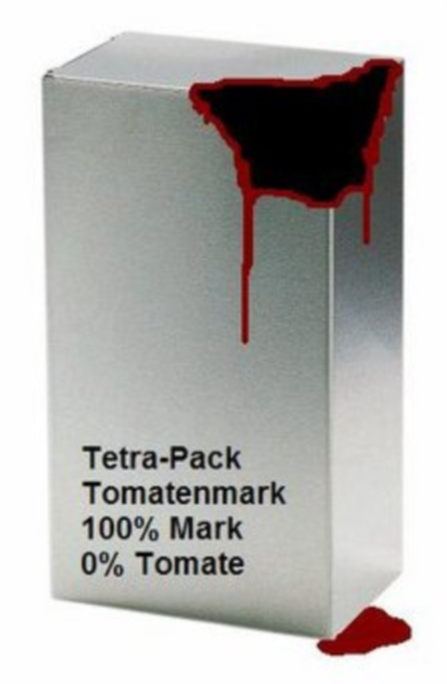
\includegraphics[width=0.618\textwidth]{pictures/Tetrapack}
\end{center}
\end{uebenv}

\clearpage

\section{Symmetrie}
Wir unterscheiden zwei Arten von Symmetrien, die bei Graphen von Funktionen auftauchen können. Diese Charakterisierungen gelten für Funktionen allgemein, nicht bloss für ganzrationale Funktionen.
\subsection{Achsialsymmetrie bezüglich y-Achse}
\begin{csatz}[Achsialsymmetrie]
Der Graph einer Funktion $f$ ist genau dann achsialsymmetrisch zur y-Achse, wenn
$$f(-x) = f(x)$$
für alle $x\in\mathbb{D}$ gilt.
\end{csatz}
\begin{proof}[Beweis]
Man veranschauliche sich den Sachverhalt an einem kleinen Bildchen.
\end{proof}

\begin{figure}[h!]
\begin{center}
\definecolor{xdxdff}{rgb}{0.49,0.49,1}
\definecolor{qqqqff}{rgb}{0,0,1}
\scalebox{0.618}{
\begin{tikzpicture}[line cap=round,line join=round,>=triangle 45,x=0.5cm,y=0.5cm]
\draw[->,color=black] (-5.9,0) -- (6.3,0);
\foreach \x in {-5,-4,-3,-2,-1,1,2,3,4,5,6}
\draw[shift={(\x,0)},color=black] (0pt,2pt) -- (0pt,-2pt);
\draw[color=black] (5.96,0.08) node [anchor=south west] {$x$};
\draw[->,color=black] (0,-3) -- (0,7.5);
\foreach \y in {-2,-1,1,2,3,4,5,6,7}
\draw[shift={(0,\y)},color=black] (2pt,0pt) -- (-2pt,0pt);
\draw[color=black] (0.1,7.02) node [anchor=west] {$y$};
\clip(-5.84,-3) rectangle (6.3,7.5);
\draw[line width=1.6pt, smooth,samples=100,domain=-5.84:6.3] plot(\x,{0.5*(\x*\x)-2});
\draw [dotted] (-4,6)-- (-4,0);
\draw [dotted] (4,0)-- (4,6);
\draw [dotted] (-4,6)-- (4,6);
\draw (-4.7,0) node[anchor=north west] {$-x$};
\draw (3.6,0) node[anchor=north west] {$x$};
\draw (4.1,3.4) node[anchor=north west] {$f(x)$};
\draw (-6.1,3.4) node[anchor=north west] {$f(-x)$};
\draw[color=black] (-5,7) node {$f$};
\fill [color=qqqqff] (4,6) circle (1.5pt);
\fill [color=xdxdff] (-4,6) circle (1.5pt);
\end{tikzpicture}
\definecolor{xdxdff}{rgb}{0.49,0.49,1}
\begin{tikzpicture}[line cap=round,line join=round,>=triangle 45,x=0.5cm,y=0.5cm]
\draw[->,color=black] (-5.8,0) -- (6.34,0);
\foreach \x in {-5,-4,-3,-2,-1,1,2,3,4,5,6}
\draw[shift={(\x,0)},color=black] (0pt,2pt) -- (0pt,-2pt);
\draw[color=black] (6,0) node [anchor=south west] {$x$};
\draw[->,color=black] (0,-4.86) -- (0,5.5);
\foreach \y in {-4,-3,-2,-1,1,2,3,4,5}
\draw[shift={(0,\y)},color=black] (2pt,0pt) -- (-2pt,0pt);
\draw[color=black] (0.1,5.1) node [anchor=west] {$y$};
\clip(-6.5,-5.2) rectangle (6.34,5.5);
\draw[line width=1.6pt, smooth,samples=100,domain=-5.8:6.34] plot(\x,{\x^3/16});
\draw [dotted] (-4,0)-- (-4,-4);
\draw [dotted] (4,0)-- (4,4);
\draw [dotted] (4,4)-- (0,4);
\draw [dotted] (-4,-4)-- (0,-4);
\draw (4.12,2.4) node[anchor=north west] {$f(x)$};
\draw (-6.5,-1.46) node[anchor=north west] {$-f(-x)$};
\draw (-4.8,1) node[anchor=north west] {$-x$};
\draw (3.6,0) node[anchor=north west] {$x$};
\draw[color=black] (-3.72,-4.9) node {$f$};
\fill [color=xdxdff] (-4,-4) circle (1.5pt);
\fill [color=xdxdff] (4,4) circle (1.5pt);
\end{tikzpicture}
}
\end{center}

\caption{Achsensymmetrie bezüglich $y$-Achse, Zentralsymmetrie zu Ursprung}
\end{figure}

\subsection{Zentralsymmetrie bezüglich Ursprung}
\begin{csatz}[Punktsymmetrie]
Der Graph einer Funktion $f$ ist genau dann punktsymmetrisch zum Ursprung, wenn
$$-f(-x) = f(x)$$
für alle $x\in\mathbb{D}$ gilt.
\end{csatz}
\begin{proof}[Beweis]
Man veranschauliche sich den Sachverhalt ebenfalls an einem kleinen Bildchen.
\end{proof}

Um das qualitative Verhalten einer Funktion besser zu verstehen, lohnt es sich, ihren Graphen zu betrachten. Dazu müsste man die Werte aus einer umfangreichen Wertetabelle in ein Koordinatensystem übertragen. In vielen Fällen kann man den Graphen schnell skizzieren, wenn man nur einige markante Punkte des Graphen kennt und untersucht, wie sich die Funktionswerte verhalten, falls die $x$-Werte gegen $\infty$ bzw. $-\infty$ streben.

\begin{uebenv}{sincostan}
Nenne eine gerade und eine ungerade Winkelfunktion.
\end{uebenv}

\begin{lsg}{sincostan}
    Man nehme beispielsweise Sinus als punktsymmetrische Funktion zum Ursprung und Cosinus als achsialsymmetrische Funktion zur $y$-Achse.
\end{lsg}

\clearpage

\section{Mathematik und Wirtschaft}

Die in den Wirtschaftswissenschaften häufig benutzten Funktionen sind
\begin{itemize}
\item Kostenfunktion $K(x)$
\item Stückkostenfunktion $k(x)=\frac{K(x)}{x}$
\item Preisfunktion $p(x)$
\item Erlösfunktion $E(x)=x\cdot p(x)$
\item Gewinnfunktion $G(x)=E(x)-K(x)$
\item Angebotsfunktion $p_A(x)$
\item Nachfragefunktion $p_N(x)$
\end{itemize}

Verändert man eine Produktion von $x_0$ Einheiten auf $x_1$ Einheiten, so entsteht ein Kostenzuwachs $\Delta K$. Der Differenzenquotient
$$\frac{\Delta K(x)}{\Delta x}=\frac{K(x_1)-K(x_0)}{x_1-x_0}$$
entspricht dem durchschnittlichen Kostenzuwachs.
Wenn die Funktion $K$ differenzierbar ist, gibt der differenzialquotient
$$K'(x_0)=\lim_{h\to0}\frac{K(x_0+h)-K(x_0)}{h}$$
die Grenzkosten, auch marginale Kosten genannt, bei der Produktion von $x_0$ Einheiten an.Durch $K'(x_0)$ erhält man die Produktionskosten für eine zusätzliche Einheit, wenn schon $x_0$ Einheiten produziert werden.
In ganz ähnlicher Weise sind marginaler Preis, Grenzerlös, Grenznutzen oder Grenzneigung zum Konsum durch Differenzialquotienten definiert. Beispielsweise gibt
$$\frac{dG(x_0)}{\mathrm{d}x}$$
in erster Näherung an, um wie viele Einheiten sich der Gewinn verändert, wenn die unabhängige Variable, die Ausbringung eines Gutes, sich um eine Einheit, von $x_0$ auf $x_0 + 1$, verändert.

\clearpage

\section{Vom Regenbogen}
Eine Extremwertaufgabe, die im Regenbogen steckt.
\marginnote{
\qrcode{
https://www.youtube.com/watch?v=tdSILv7E7t4}
}


\cleardoublepage
\listoffigures
\listoftables

\end{document}